\documentclass[11pt]{article}
\usepackage[margin=1in]{geometry}
\usepackage{amsmath,amssymb}
\usepackage{booktabs}
\usepackage{hyperref}
\usepackage{enumitem}
\usepackage{xcolor}
\usepackage{graphicx}

\hypersetup{colorlinks=true, linkcolor=blue, citecolor=blue, urlcolor=blue}

\title{Supplementary route ledgers for Paper 10}
\author{Jozsef Olcsak}
\date{Supplementary audit source}

\begin{document}
\maketitle

\section*{Scope}

This supplement preserves the detailed route-by-route audit trail that was
moved out of the main Paper 10 text to keep the main manuscript readable.  The
supplement records source products, review packages, replay permissions,
control outcomes, and negative-route diagnostics.  It does not strengthen any
claim beyond the main paper: the status remains prevalidation and not a joint
cosmological likelihood.

\section{Data blocks}

The intended public data blocks are summarized in
Table~\ref{tab:data-blocks}. The table is a work order, not a completed
measurement.

\begin{table}[h]
\centering
\small
\begin{tabular}{lll}
\toprule
Block & Candidate public sources & Role \\
\midrule
Distance & DESI BAO, SNe, \(H(z)\), CMB priors & test \(E_D(z)\) \\
Void maturity & void catalogues & freeze \(W_V(a)\) \\
Web anisotropy & cosmic-web classifiers & freeze \(W_W(a)\), \(Q_{\rm env}\) \\
Growth & RSD \(f\sigma_8\), clustering & test \(\mu_\tau\) \\
Lensing & weak lensing, CMB lensing, cluster lensing & test \(\Sigma_{\rm lens}\) \\
CMB safety & Planck/LAMBDA products & early safety and lensing controls \\
\bottomrule
\end{tabular}
\caption{Planned source blocks for the Friedmann-readout audit. DESI data
products~\cite{DESIDR2BAO2025,DESIDR2Products2025}, Planck products
~\cite{Planck2018Cosmology,PlanckLegacyArchive}, and NASA LAMBDA
~\cite{NASALAMBDA}, the public Cosmic Chronometers data page
~\cite{CosmicChronometersData}, SDSS cosmic-web and eBOSS/LSS products
~\cite{SDSSCosmicWebVAC,SDSSDR16LSS}, and KiDS-1000 lensing products
~\cite{KiDS1000Lensing} are examples of public source routes.}
\label{tab:data-blocks}
\end{table}

The repository also contains a source-freeze manifest:
\[
\texttt{data/source\_manifest/paper10\_source\_freeze\_manifest.csv}.
\]
It records candidate public source families, whether the source has merely been
selected or remains blocked, the planned local artifact path, and the endpoint
fields forbidden during source selection. In the current manifest, the first
source-selection audit has identified candidate public source routes for all
required blocks, but no source row is yet \texttt{FETCHED\_FROZEN}. This is the
key distinction: source-family selection is not endpoint readiness. These
blocks cannot be used for endpoint scoring until the public source product,
version, transformation rule, and checksum policy are frozen.

\section{Leakage prevention}

The audit follows a source-freeze discipline:

\begin{enumerate}[leftmargin=1.5em]
\item Freeze void maturity \(W_V\) before distance residual scoring.
\item Freeze web anisotropy \(W_W\) and \(Q_{\rm env}\) before growth/lensing scoring.
\item Keep CMB primary maps as early-safety and consistency controls.
\item Run shuffled environment labels and wrong-proxy nulls.
\item Do not use target residuals to choose activation functions.
\end{enumerate}

This is the cosmological analogue of the matched-vs-wrong and non-overlap
ledger discipline used in Papers 8 and 9.

In the current scaffold, the validation script
\(\texttt{scripts/validate\_source\_freeze.py}\) checks that the manifest covers
the required blocks and explicitly forbids endpoint leakage fields such as
distance residuals, growth residuals, lensing residuals, fit-improvement flags,
and post-hoc environment labels. Passing this script is not a data result; it is
a precondition for a later real-data pilot.

The repository further includes a compact provenance cache of the official
source landing pages. The acquisition script
\(\texttt{scripts/acquire\_source\_pages.py}\) records the landing-page payloads,
byte counts, and SHA-256 hashes, while
\(\texttt{scripts/validate\_cached\_source\_pages.py}\) verifies the committed
cache during reproduction. These cached pages are not raw survey products and
are not used to compute cosmological observables; they only make the source
routes auditable without requiring live network access during reproduction.

A second preflight artifact,
\(\texttt{data/source\_manifest/paper10\_product\_freeze\_plan.csv}\),
declares the product role, planned local path, transformation-rule identifier,
covariance policy, mask or selection policy, and forbidden endpoint fields for
each source family. In this scaffold every product row has
\(\texttt{endpoint\_allowed=false}\). Thus the protocol now specifies the next
data-acquisition step, but still does not contain endpoint data or a
measurement result.

The next void/web-specific preflight artifact is a source-native freeze plan.
It selects a preferred source-native void route through a VAST/SDSS DR7 archive
candidate~\cite{VASTSDSSDR7VoidZenodo} and a preferred web route through the
SDSS DR17 MCPM cosmic-web catalogue identified by the SDSS value-added
catalogue page~\cite{SDSSCosmicWebVAC}. This artifact exists because the
current \(W_{\rm void}+W_{\rm web}\) pilot still uses redshift/scale-factor
proxy bases. The rows in this new plan are selected but not fetched, and
endpoint scoring remains disabled; they freeze candidate routes, not numerical
endpoint inputs.

After that route-selection gate, the current repository also freezes the first
source-native void/web products. The void side contains a VAST/SDSS DR7
Planck2018 maximal void table with 1163 rows and its NSA mask. The web side
contains the SDSS DR17 MCPM SlimeMold galaxy catalogue. Its first FITS table
extension contains 638820 rows, and the provider sha1sum file is frozen as an
additional provenance check. These files are checksum-locked and source-native,
but still not endpoint inputs: the transform from catalogue quantities to
\(W_{\rm void}\) and \(W_{\rm web}\) scoring columns remains a future frozen
gate.

The current package then adds that first transform as a separate non-scoring
design-matrix step. It maps the maximal-void catalogue to a cumulative
source-only void load and the MCPM catalogue to a redshift-binned web-density
load. In the retained Pantheon+ scope, 426 rows receive nonzero void support and
1333 rows receive nonzero web support. A separate source-native full-covariance
pilot can score these columns under the same distance-only grammar. It improves
\(\chi^2\) by \(0.508\) relative to the flat-\(\Lambda\)CDM branch, but loses
under AIC by \(3.49\), and the deterministic shuffled control still reaches a
lower \(\chi^2\). This is therefore a useful source-native pipeline step, not a
void/web detection and not endpoint validation.

The first growth-side extension freezes six SDSS final BAO/RSD
\(f\sigma_8(z)\) summary points from the public SDSS final-measurements table
and attaches the source-native \(W_{\rm web}\) basis to those redshifts. This
diagonal-summary pilot improves \(\chi^2\) by \(0.306\) relative to a simple
growth-index \(\Lambda\)CDM branch, but loses under AIC by \(1.69\). The
wrong-sign control is equally good on the symmetric pilot grid, so the run does
not establish a preferred web direction. Its value is narrower: it shows how
the web channel enters a growth-side observable and why the next real gate must
use the official compressed-parameter covariance or a fuller RSD likelihood.

That next covariance gate is included as a separate SDSS multi-tracer
BAO/RSD pilot. The repository fetches and hash-locks the official DR16
LRG+ELG compressed BAO/RSD products and uses the Fourier-space six-component
vector
\[
\{D_M/r_d,D_H/r_d,f\sigma_8\}_{z=0.70,0.845}
\]
with its published \(6\times6\) covariance. In this pilot \(W_{\rm web}\)
acts only on the two growth entries, while the BAO entries remain in the
shared covariance block. The result is essentially neutral: the web branch
improves \(\chi^2\) by only \(0.010\), loses under AIC by \(1.99\), and the
wrong-sign control reaches the same best \(\chi^2\). This is therefore a useful
multi-probe covariance check and seminegative control, not evidence for a
preferred web-growth direction.

After the FLRW-consistency audit, the repository records these source-native
distance and growth pilots in a separate void/web endpoint-readiness ledger.
The ledger has four components: Pantheon distance, SDSS growth, SDSS
multi-tracer BAO/RSD, and CMB safety. It records no endpoint-ready scoring
component. The CMB-safety component passes only as a known-limit support check;
the scoring-facing components remain blocked by AIC loss, shuffled or
wrong-sign controls, and near-zero full-covariance signal. The next legitimate
void/web step is therefore a predeclared combined multiblock endpoint protocol
with joint null controls and a unified information criterion, not promotion of
any isolated pilot.
That protocol is now frozen only as a shell: the active families are
\(W_{\rm void}\) and \(W_{\rm web}\), \(W_{\rm path}\) and \(W_{\rm time}\)
remain disabled, and the future score must combine distance, growth, and
multi-tracer covariance blocks under a shared information criterion with
block-drop and shuffled/wrong-family controls. No combined likelihood or
endpoint score is computed in the present paper.
A separate authorization-review template is also frozen. It remains
uncompleted and keeps endpoint execution disabled; a future combined run
requires an accepted permission-only response based on the protocol and
source-side readiness artifacts, not on residuals or fit statistics.

The first CMB-safety artifact is even narrower. It is not a CMB likelihood and
does not use CMB maps. It only asks whether the currently active late-time
void/web source-native bases vanish outside their low-redshift support. Using a
conservative safety floor \(z=10\) and a recombination proxy \(z=1089.92\), the
check finds
\[
W_{\rm void}(z)=W_{\rm web}(z)=0
\]
at both probe redshifts. This is a known-limit sanity check: the present
late-time pilots do not directly modify the early-universe CMB-safety regime.
It is not evidence for a CMB-detected Tau Core effect.

The lensing block is advanced only to a route-freeze stage. The repository
records the public KiDS-1000 cosmic-shear tarball route and verifies its HEAD
metadata, including availability, content type, and content length. It does not
fetch or redistribute the tarball and contains no KiDS data vector, covariance
matrix, posterior chain, lensing residual, or fit statistic. A future lensing
pilot must first freeze the tomographic-bin policy, statistic choice
\((\mathrm{COSEBIs},\xi_\pm,\mathrm{bandpowers})\), covariance block, mask
policy, and readout policy before any \(W_{\rm web}\) or \(W_{\rm path}\)
lensing score can be interpreted.

The next lensing preflight step then checksum-locks the KiDS-1000 cosmic-shear
tarball and builds a non-scoring inventory. The tarball contains three FITS
summary-statistic products, and the route selects exactly one source-side
COSEBIs FITS member as the first narrow future lensing statistic route. This is
motivated by the KiDS release documentation, which identifies COSEBIs as the
fiducial analysis statistic for the cosmic-shear products. The artifact remains
endpoint disabled: it records file membership and the future COSEBIs route, not
a lensing likelihood or a Tau Core lensing score.

Finally, the selected COSEBIs FITS product is inspected at the HDU-policy level.
The frozen roles are \( \mathrm{COVMAT} \) for the \(300\times300\) covariance
matrix, \(\mathrm{En}\) for the 300-row COSEBIs data-vector table, and
\(\mathrm{NZ\_SOURCE}\) for the 119-row source redshift-distribution table.
The covariance is positive definite. This closes the first source-side
lensing-survival route down to an identifiable statistic and covariance block,
but it still does not define a theory prediction, likelihood, residual, or Tau
Core lensing amplitude.

The COSEBIs data-vector structure is then frozen at the tomographic/mode level.
The selected \(\mathrm{En}\) table contains five source bins, 15
upper-triangular tomographic bin pairs, and 20 COSEBIs modes per pair, for 300
data-vector rows. This closes the source-side pair/mode inventory required by a
future lensing pilot, but still does not choose a mode cut, invert the
covariance, define a theory vector, or score any \(W_{\rm web}\) or
\(W_{\rm path}\) lensing residual.

The covariance block is separately audited as a readiness object. The selected
\(\mathrm{COVMAT}\) matrix is checked for shape, symmetry, positive diagonal,
eigenvalue spectrum, condition number, and Cholesky readiness. No inverse
covariance is saved, and no likelihood is evaluated. Thus the lensing route now
has a source-side statistic, data-vector structure, and covariance-readiness
record, but it remains below the endpoint threshold until the theory-vector,
mode-cut, mask, tomographic-weight, and covariance-inversion policies are
predeclared.

The first mask/mode-cut policy is intentionally conservative: all 300
source-side COSEBIs rows are retained, covering all 15 tomographic pairs and
modes \(1,\ldots,20\). No row, tomographic pair, or mode is removed using
endpoint residuals, fit statistics, posterior chains, or model-performance
information. This makes the later lensing route more restrictive rather than
more flexible: any future physically motivated cut must be declared in a new
source-side policy before scoring.

The tomographic-pair retention weights are likewise frozen to a neutral
pre-score rule: every retained pair receives unit source-retention weight. These
are not likelihood weights and not fitted amplitudes. They only record that no
tomographic pair is upweighted or downweighted using endpoint residuals,
posterior chains, or fit-improvement information. Statistical coupling remains
reserved for a future predeclared covariance-inversion policy.

The covariance-subselection policy then retains the full \(300\times300\)
covariance block. It records the contiguous 20-row covariance intervals
corresponding to each retained tomographic pair, but removes no covariance rows
or columns. No inverse covariance is saved at this stage. This keeps the lensing
route source-complete while still below the likelihood endpoint.

The covariance-inversion policy is also frozen, but only as a future numerical
method: a Cholesky solve against the full covariance, without materializing or
storing an inverse covariance matrix. The endpoint-family geometry gate is now
resolved below, but the solve is still not executed in the present artifact
because the lensing scoring protocol remains a frozen-not-run shell.

The theory-vector gate is declared next. Its parent policy remains
endpoint-disabled and declarative: it fixes the future target length to the 300
retained COSEBIs rows and keeps the lensing route restricted to \(W_{\rm web}\)
and \(W_{\rm path}\), while forbidding use of KiDS data-vector values, posterior
chains, residuals, or fit-improvement flags to choose the vector. A separate
source-frozen unit-amplitude shell is then built from the frozen mapping basis
and a predeclared unit-mean \(n^{-1/2}\) mode-shape rule. This is still not a
prediction: it contains no residual, likelihood, AIC value, null-control score,
or endpoint validation.
The companion template materializes the 300-row tomographic-pair/mode interface
and freezes row order before the source-frozen shell is assembled.

The web/path mapping gate is also declared but not computed. It requires future
source-frozen web-environment, lensing-path mask or depth-map, redshift-kernel,
and null sky-rotation or pair-shuffle products before a COSEBIs theory vector
can be constructed. The mapping policy explicitly forbids KiDS data-vector
values, posterior chains, residuals, fit-improvement flags, and post-hoc sky
direction choices.

One of those required source products is then advanced from a declaration to a
source-side inventory: the selected \(\mathrm{NZ\_SOURCE}\) table is read to
record the redshift-distribution area, mean redshift, and support interval of
each of the five KiDS source bins. This redshift-kernel inventory is not a
lensing prediction. It does not evaluate a COSEBIs theory vector, does not
reweight bins using endpoint behavior, and does not use the KiDS data-vector
values, residuals, posterior chains, or fit statistics.

The path-projection input is treated more conservatively. A source-side gap
audit scans the selected KiDS-1000 cosmic-shear release tarball and records no
accepted standalone footprint, depth map, survey mask map, random catalogue, or
equivalent path-load product. The word ``mask'' appears in the statistic FITS
filenames, but this is not accepted as a survey path map. Thus the
\(W_{\rm path}\) lensing route remains blocked on an external source-frozen
path/mask/depth product before any path-aware COSEBIs theory vector can be
constructed.
The next route-freeze step identifies the official KiDS DR4 mask-script route:
the preferred DR4.1 nine-band mask wget script is hash-frozen and lists 196
external mask FITS products. Those FITS products are not downloaded in the
present package, and no mask map or path-mapping vector is parsed. This narrows
the blocker from an unknown missing product to a source-frozen external mask
route.
The preferred route is then parsed into a 196-tile filename-coordinate
inventory. This gives a source-frozen route geometry index, but still not a
survey footprint polygon, pixel-level path weight, COSEBIs row assignment, or
theory vector.
A first route-health check then performs HEAD requests for the first, middle,
and last mask products in the preferred route. All three return HTTP 200 with
FITS content and positive content length. This is still only metadata: no mask
FITS file is downloaded and no path-aware lensing theory vector is constructed.
The same predeclared first/middle/last sample is then materialized as a tiny
source-side mask subset. The three downloaded mask FITS products are hash-frozen
and parsed only to record image shapes and finite/nonzero pixel summaries. This
establishes that the route can supply actual mask images, but it still does not
construct a \(W_{\rm path}\) mapping, connect mask pixels to the 300 COSEBIs
rows, or evaluate any lensing score.
From this subset we build only a source-observable shell: filename-derived tile
coordinates plus a centered zero-fraction shell across the three frozen masks.
The mask-value semantics are not interpreted as physical lensing path weights in
this gate. The shell is therefore a pre-mapping observable, not a COSEBIs
mapping vector, theory vector, or endpoint likelihood input.
We then assemble a 300-row design skeleton: each COSEBIs target row carries its
tomographic pair, mode index, the relevant source-bin redshift summaries, and
the preferred-route sky span. This is still only a layout. No tile/path weight,
mapping-vector element, or theory-vector element is evaluated.
Finally, the design layout is expanded to the full target-row by route-tile
domain of \(300\times 196=58{,}800\) rows. This freezes the future mapping
domain without assigning footprint overlap, depth/path weight, web-environment
label, mapping-vector element, or likelihood contribution.
The admissible future weight rule is then declared symbolically as a product of
redshift-pair, route-tile, footprint-overlap, path/depth, web-environment, and
normalization factors. This rule is not yet computable: the footprint-overlap
and web-environment factors are missing, the path/depth factor is only a
three-mask partial shell, and no numeric weight is produced.
The corresponding acquisition plan turns this into concrete source-side
requirements: obtain or derive a footprint/row-tile overlap rule, promote the
path/depth factor beyond the three-mask shell, attach a source-frozen
web-environment catalogue or predeclared null-web control, and define the
normalization only after nonzero source factors exist. No products are fetched
and no factors are evaluated in this gate.
We also freeze a source-product route manifest for the next step. It lists ten
candidate routes: two already-supported locks, five blocker-resolution
candidates, and three control/deferred routes. This manifest is still
source-side only: it fetches no products, computes no factor values, and does
not construct a path mapping or score.
Finally, a blocker-resolution order policy fixes the future source-side order:
footprint overlap first, then path/depth support, web/environment support,
normalization, mapping-vector construction, and null controls. Thus later
normalization or null-control steps cannot bypass the missing footprint
support.
For the first blocker, a \texttt{F\_overlap} shell declares the future accepted schema:
one source-frozen support row per COSEBIs target-row by route-tile domain entry
over the full $300\times196=58{,}800$ domain. The shell accepts official
footprint geometry or source-native full-mask overlap derivations, but computes
no overlap values in this paper.
The corresponding availability audit preserves the current negative state: the
route script and the three-mask subset are present, but neither an accepted
official footprint geometry product nor a full 196-mask source-native product
set is available. Therefore \texttt{F\_overlap} remains unresolved.
The full-mask acquisition manifest makes this explicit at tile level: three
mask products are locally present and 193 remain missing.
These missing products are split into ten future acquisition batches, with
large FITS products assigned to an ignored cache rather than to the committed
paper repository.
A first batch dry run then inspects batch 0, containing 20 planned product URLs
and cache paths, without downloading any FITS file. The dry run is included in
the public reproduction script, while the manual \texttt{--execute} acquisition
mode is kept outside the public reproduce path and writes only to ignored local
execution logs. This gate computes no overlap fraction, path-mapping vector,
theory vector, prediction, residual, or endpoint score; it is only a
leakage-safe acquisition-readiness check.
The following batch-promotion checklist is deliberately negative in the current
release: no fetched-batch review artifact, checksum manifest, complete batch
accounting, or forbidden-input audit has been committed. The checklist therefore
keeps promotion disabled and does not read ignored local execution logs. Passing
such a checklist in the future would still not be an overlap rule; it would only
make a fetched batch eligible for a separate source-native overlap derivation.
The checklist now records the filled-review validator as available, but this is
only a future-review readiness condition and does not change the present
negative promotion status.
To make that future step auditable, the repository also freezes the required
schema for a fetched-batch execution-review artifact: product identity, URL,
cache path, HTTP status, byte count, SHA-256, review status, reviewer role,
forbidden-input flags, and claim-boundary flags. This is a schema declaration
only; no fetched-batch review artifact is present in the current release.
An empty batch-0 template is also materialized in that schema. It contains the
20 planned product rows, but no network status, checksum, timestamp, reviewer
entry, or source-freeze decision. It is therefore a review template, not an
execution log.
A separate filled-review validator is provided to check this template, or a
future manually completed execution-review artifact, against the frozen schema
and dry-run batch identities. This validator is not a promotion gate and does
not compute an overlap rule, mapping vector, theory vector, prediction,
residual, or score.
The corresponding F-overlap resolution decision records that no endpoint-grade
overlap route is accepted yet: the three source-frozen masks are retained only
as a caveated partial path-mask control, while the official-geometry,
full-196-mask, and batch-0 dry-run routes remain unresolved.
A separate partial-control scoring protocol freezes only a future diagnostic
grammar for that caveated three-mask control. It does not run scoring, emit
score artifacts, or create a population endpoint claim.
The accompanying partial-control mapping shell materializes only the
\(300\times3=900\) source-side support table connecting COSEBIs rows to the
three caveated mask controls; it computes no mapping value, theory vector,
residual, or score.
A further source-only diagnostic artifact freezes partial-control mapping
values on this same support table using
\[
  m_{\rm pc} =
  s_{\rm mask}\,
  w_{\bar z}(i,j)\,
  n^{-1/2},
\]
where \(s_{\rm mask}\) is the three-mask shell value, \(w_{\bar z}(i,j)\) is a
normalized mean-redshift pair weight from the KiDS \(NZ\_SOURCE\) inventory,
and \(n\) is the COSEBIs mode index. This is a caveated partial-control
mapping-value artifact only: it is not an endpoint mapping vector, not a
COSEBIs theory vector, and it computes no residual, likelihood, score, or
validation statistic.
The next scoring-facing, still non-scoring object is a partial-control design
matrix: the \(900\) mapping values are reduced to six deterministic 300-row
branches, namely a zero baseline, the three individual mask-sample branches, a
positive-mask mean, and a sign-flipped positive-mask control. This design
matrix is not an endpoint theory vector. It is only the branch interface that a
future diagnostic partial-control score would use after a separate scoring
protocol is opened.
We then run that caveated diagnostic score, still outside endpoint validation.
The retained KiDS COSEBIs \(En\) vector is compared to each predeclared branch
using the full \(300\times300\) covariance and a nonnegative one-amplitude rule.
The best positive-mask branch lowers the diagnostic \(\chi^2\) by about
\(183.6\) relative to the zero branch. This number is not a KiDS endpoint
claim: in this simplified three-mask control the positive branches are
amplitude-degenerate, and the run is included only as a scoring-pipeline smoke
test showing that the partial-control route can be evaluated without changing
source labels, branch labels, masks, weights, or mode cuts after seeing
residuals.
We then replay the observed positive-mask diagnostic branch against \(1008\)
deterministic null controls: sky rotations, tomographic-pair shuffles,
wrong-channel activations, and sign-flip controls. One tomographic-pair shuffle
slightly outperforms the observed branch, so the observed branch is not an
absolute winner. The conservative plus-one tail fraction is \(0.001982160555\).
This is retained only as a diagnostic rarity check for the caveated
partial-control route, not as endpoint validation and not as a KiDS lensing
population claim.
Finally, before promoting any such branch to an endpoint route, we audit the
branch geometry itself without using the KiDS \(En\) data vector. The positive
partial-control branches are effectively rank one: their covariance-metric
absolute cosine is numerically unity and the maximum positive-branch relative
shape residual is about \(2.2\times10^{-12}\). This audit is a useful negative
result. It explains why the diagnostic score can be interesting while still
being insufficient for endpoint evidence: the three-mask branch family must be
replaced by a non-degenerate, source-frozen full-route or official-geometry
mapping before endpoint scoring.
We therefore add a non-degenerate mapping promotion gate. It freezes six
conditions before any endpoint promotion is allowed: endpoint-grade
\texttt{F\_overlap}, source-preflight readiness, endpoint-family geometry, a
frozen 300-row theory vector, null controls after mapping, and leakage guards.
The earlier positive partial-control branch remains rank one and is preserved
as a negative diagnostic result. It is not used as the endpoint family. Instead
we audit the source-frozen candidate theory shell together with the
predeclared source-frozen null-control theory replay. This endpoint comparison
family contains \(1009\) vectors over the \(300\) retained COSEBIs rows and has
effective rank \(15\) in both the raw Euclidean and covariance-metric geometry
audits. The geometry audit uses the KiDS covariance only as a metric; it does
not read the KiDS \(E_n\) data-vector values, residuals, posterior chains, fit
statistics, or endpoint scores. With this replacement, all six promotion gates
pass. Endpoint scoring remains disabled because no explicit endpoint scoring
run is executed in this release.
The scoring-facing view is then summarized by an endpoint-readiness ledger:
the COSEBIs data-vector structure, covariance matrix, covariance solve policy,
theory-vector row-interface template, mapping-to-template join contract,
F-overlap resolution/control decision, web/path source mapping, source-preflight
mapping basis, and source-frozen unit-amplitude theory-vector shell are
source-side ready. The predeclared null controls have also been replayed against
the source-frozen theory shell as deterministic control-vector digests, without
computing null scores. After the endpoint-family geometry audit, the readiness
ledger records twelve ready components and no remaining readiness blocker.
A corresponding scoring-protocol shell freezes only the future grammar
\(\chi^2=(d-t)^T C^{-1}(d-t)\), with a Cholesky covariance solve and required
baseline, candidate, wrong-channel, shuffled/rotated null, AIC, and control-rank
outputs. The protocol shell itself is not a likelihood run. After explicit
approval, the first endpoint scoring run applies this frozen grammar to the
retained 300-row KiDS COSEBIs \(E_n\) vector. The source-frozen candidate
improves on the zero baseline by
\[
  \Delta\chi^2=-183.6152665217,
  \qquad
  \Delta{\rm AIC}=-181.6152665217,
\]
using the full covariance Cholesky solve and a nonnegative single-amplitude
branch rule. Against the 1008 predeclared null-control vectors, the candidate
ranks \(3/1009\) by both \(\chi^2\) and AIC, giving a plus-one null-tail
fraction \(0.002973240832507\). This is a KiDS endpoint score, not validation:
the KiDS data vector enters only after source-side choices, candidate vectors,
and null controls are frozen, and two predeclared null controls still score
better than the candidate.
The post-score diagnostic localizes this caveat: both better controls are
tomographic-pair shuffles, while the sky-rotation, wrong-channel, and sign-flip
control families do not beat the candidate. The next robustness question is
therefore whether the signal is stable to stricter tomographic-pair structure
tests, not whether it is explained by a generic wrong-channel activation.
A follow-up robustness run answers this in the same claim-safe sense. Against
all \(119\) non-identity five-bin label permutations and \(1000\)
auto/cross-preserving pair shuffles, the candidate ranks \(4/1120\), with
plus-one tail fraction \(0.003571428571429\). Three structured controls beat
the candidate, so this still is not validation, but the low-tail behavior
survives a stricter tomographic-structure null ensemble.
We then audit whether the better tomographic controls are plausible physical
alternatives. The top-control plausibility ledger reads the top 25 controls and
the source-side redshift kernel inventory, but computes no new score. The three
better controls are classified as two control-only non-global pair shuffles and
one conditional source-systematic candidate that would require independent
photometric-redshift or tomographic-calibration support. Thus the controls do
not refute the endpoint signal in the present source state, but they do block a
validation claim.
We therefore freeze a tomographic holdout/calibration gate before any further
endpoint replay. This gate computes no new score and authorizes no replay. It
requires, first, independent photometric-redshift or tomographic-calibration
evidence; second, a source-bin or tomographic-pair holdout partition fixed
before scoring; third, a source-side rule for when a tomographic control may be
promoted to a calibration-systematic candidate; fourth, a frozen replay
protocol; and fifth, a leakage validator. Observed COSEBIs values, endpoint
residuals, \(\Delta\chi^2\), null-control ranks, best-control identity, and
post-score residual shape are forbidden source-selection inputs. The resulting
gate verdict is that a tomographic holdout is required before endpoint replay
or validation.
As the first non-scoring response to that gate, we freeze a deterministic
source-bin holdout manifest. The manifest uses only the committed
source-native redshift-kernel inventory: in fold \(k\), all tomographic pairs
that touch source bin \(k\) are held out and all remaining pairs are
calibration pairs. This freezes the holdout partition but does not complete the
independent-calibration requirement. Endpoint replay therefore remains
forbidden until independent photometric-redshift or tomographic-calibration
evidence is attached.
We also add a source-side photo-\(z\)/tomographic evidence ledger. It accepts
the checksum-frozen KiDS lensing tarball, cached KiDS DR4 lensing-page
photo-\(z\)/SOM-gold documentation markers, and the source-native
\texttt{NZ\_SOURCE} five-bin inventory, but it keeps independent external
photo-\(z\) or tomographic calibration open. This ledger computes no new score
and does not authorize endpoint replay.
Finally, we freeze a source-side acquisition plan for the missing H1 evidence:
an external photo-\(z\) calibration reference or product manifest, an
independent SOM-gold or redshift-distribution validation manifest,
tomographic-bin quality or \(\Delta z\) prior evidence, and a leakage review
for any attached calibration artifact. At the acquisition-plan stage no route
was attached, so H1 remained open and endpoint replay remained forbidden.
We then attach cached public sources for the first three H1 routes: the
KiDS-1000 redshift-calibration article, its arXiv metadata page, and the
official KiDS DR4 SOM-gold catalogue page. These sources support the
photo-\(z\)/\(n(z)\), SOM-gold, five-bin tomographic, and clustering-redshift
calibration context. An automated leakage-review preflight then checks that the
attached source artifacts and their manifest builder do not use endpoint
residuals, endpoint scores, post-score ranks, or fit statistics. This automated
preflight passes, but it is not an independent reviewer attestation. At this
handoff stage the full R4 leakage review route therefore remained open, H1 was
not yet complete, and endpoint replay remained forbidden. We also provide a
blank independent reviewer attestation template that states the source-side
questions and forbidden endpoint fields for the remaining R4 step; it is a
handoff artifact, not a completed review response.
A completed source-side reviewer response was then imported and validated. The
response accepts the R4 leakage review as caveated source-side evidence, marks
the independent reviewer attestation, R4 leakage review, and H1 external
photo-\(z\)/tomographic-calibration evidence gates as source-side complete, and
explicitly keeps \texttt{endpoint\_replay\_allowed=false} and
\texttt{endpoint\_validation\_claimed=false}. A separate closure ledger records
this current post-reviewer source-side state. The ledger does not rewrite the
earlier prerequisite artifacts, does not compute new endpoint scores, and does
not authorize endpoint replay; any future endpoint replay requires a separate
explicit human authorization gate.
A separate endpoint-replay authorization response was then validated. It gives
\texttt{GO\_SOURCE\_SIDE\_REPLAY\_PERMISSION\_ONLY} for one predeclared replay
under the existing frozen source-side state, while keeping
\texttt{forbidden\_inputs\_used=false} and
\texttt{endpoint\_validation\_claimed=false}. This changes the replay permission
state only; it does not promote the KiDS endpoint to validation.
Under this permission-only gate the endpoint replay reproduces the frozen
COSEBIs result: \(\Delta\chi^2=-183.6152665217\), \(\Delta{\rm AIC}=-181.6152665217\),
candidate rank \(3/1009\) against the predeclared null controls, and plus-one
tail fraction \(0.002973240832507\). The replay summary keeps
\texttt{endpoint\_validation\_claimed=false}, so the claim-safe reading remains a
low-tail endpoint signal, not KiDS validation.
A post-replay tomographic-control disambiguation ledger then classifies the
three tomographic controls that beat the candidate in the stricter
tomographic-structure robustness ensemble. Two are control-only
non-global relabel or pair-shuffle controls, one is only a conditional
source-systematic candidate requiring independent photo-\(z\) or tomographic
support, and none is accepted as a physical alternative. This ledger computes
no new endpoint score and keeps
\texttt{endpoint\_validation\_claimed=false}. The resulting status is therefore
that the tomographic controls block validation but do not refute the low-tail
endpoint signal.
A source-frozen tomographic holdout replay gives the next diagnostic check. For
each of the five source-bin folds, the nonnegative amplitude is frozen using
only calibration tomographic pairs that do not touch the held-out source bin,
and the held-out pairs are then scored. The candidate improves over the zero
baseline in \(4/5\) held-out folds, with aggregate holdout
\(\Delta\chi^2=-521.8035067179\). However, one of the candidate-beating
tomographic controls remains slightly better in the same replay. Thus the
holdout replay preserves the low-tail signal diagnostically, but it does not
remove the tomographic-control caveat and does not constitute KiDS validation.
A final narrow source-evidence gate audits this remaining holdout-beating
control, \texttt{seeded\_auto\_cross\_shuffle\_702759}. The mapping is not
induced by a single global source-bin relabel: its auto-pair map would imply
\(1\mapsto2\) and \(2\mapsto3\), so a global relabel would send
\(1\text{--}2\) to \(2\text{--}3\), while the observed control sends
\(1\text{--}2\) to \(1\text{--}5\). With no independent photo-\(z\) or
tomographic source evidence attached, this best holdout-beating control remains
control-only rather than a physical alternative. It therefore does not refute
the endpoint signal, although the broader tomographic-control caveat continues
to block validation.
A validation-readiness ledger then summarizes the current state without
computing any new score. The allowed current claim is
\texttt{diagnostic\_low\_tail\_signal\_with\_reduced\_tomographic\_control\_concern\_not\_validation}.
The signal has survived the narrow follow-up checks performed so far, and the
most dangerous tomographic control is not accepted as a physical alternative.
Nevertheless, \texttt{validation\_ready=false}: the tomographic caveat remains
active, and physical promotion remains blocked by open
operator/amplitude/normalization requirements.
We then add a narrower tomographic/photo-\(z\) closure-status ledger. This
ledger uses the completed external photo-\(z\) reviewer response and records
\texttt{h1\_independent\_evidence\_complete=true} and
\texttt{r4\_leakage\_review\_complete=true} for the source-side photo-\(z\)
route. It therefore reduces the photo-\(z\)/tomographic source-side concern.
However, it computes no new score and does not change the validation boundary:
the source-bin holdout remains diagnostic, the best holdout-beating control is
still not promoted to a physical alternative, and
\texttt{validation\_ready=false} until the physical-promotion blockers are
closed.
We also freeze a physical-promotion dependency-order ledger. This ledger does
not prove the missing theorems; it only orders them. The next primary proof gate
is the operator-leakage theorem, and the next parallel gate is gauge/quotient
descent. Response-unit normalization, the standard-lensing/no-Tau-source
null-amplitude theorem, and the full survey-native operator theorem are
downstream of those two gates. Thus the next theory-side step is not another
endpoint score but leakage and quotient control.
For the leakage branch, we freeze a proof-plan ledger rather than a theorem.
The uniform tile-average null limit is already available, and the
no-endpoint-feedback guard is satisfied. The open exit conditions are:
non-uniform leakage projection, pure-mask quotient/control, and single-operator
coupling between the mode-response spectrum and null descent. The resulting
verdict is
\texttt{B2\_operator\_leakage\_exit\_conditions\_frozen\_but\_theorem\_open}.
For the first of these open steps, we freeze a sufficient non-uniform leakage
projection criterion. If \(V_{\rm source}\) is decomposed into candidate
physical, mask-only, and control/null subspaces, then a future operator \(O\)
must either satisfy \(\Pi_{\rm phys} O m=0\) for every mask-only direction \(m\)
modulo quotient-null directions, or route \(O(V_{\rm mask})\) into a
predeclared null-control family. This criterion is not yet proven for the KiDS
operator; its current verdict is
\texttt{nonuniform\_leakage\_projection\_criterion\_frozen\_but\_not\_proven}.
The component split itself is now declared only as bookkeeping:
\(V_{\rm phys,cand}\) denotes the source-frozen low-mode candidate response
shell, \(V_{\rm mask}\) denotes the pure-mask/depth/path basis, and
\(V_{\rm ctrl/null}\) denotes the predeclared null-control family. This changes
the \(C1\) status from definition-required to declared, but does not prove
pairwise orthogonality, quotient triviality, null projection, control routing,
or single-operator consistency. Its machine-readable verdict records that the
domain decomposition is declared, while the projection and leakage theorem
remain open.
A second post-score localization audit keeps the same source-frozen theory
vector and same nonnegative single-amplitude scoring rule, but evaluates
predeclared jackknife masks. All \(20/20\) leave-one source-bin and
leave-one tomographic-pair subsets retain negative \(\Delta\chi^2\) and
negative \(\Delta{\rm AIC}\). Thus the endpoint score is not carried by one
single source bin or one single tomographic pair under this first jackknife.
The mode-band result remains caveated: only \(2/3\) mode-only subsets improve,
and removing the low \(n=1\ldots5\) COSEBIs modes leaves no improvement over the
zero baseline. This strengthens localization robustness but does not promote
the result to KiDS validation.
A final mode-localization audit sharpens that caveat. Scoring the predeclared
single-mode, cumulative-low-mode, and low-mode-removal subsets shows that the
best single mode is \(n=1\), with
\(\Delta\chi^2=-101.5735188246\), while the strongest cumulative subset is
\(n=1\ldots3\), with \(\Delta\chi^2=-237.1074068478\). All cumulative
low-mode subsets improve, but removing the first five modes gives
\(\Delta\chi^2=0\). The endpoint signal is therefore not single-bin or
single-pair localized, but it is strongly low-mode localized. This is a
diagnostic localization result, not a validation claim.

\begin{figure}[t]
\centering
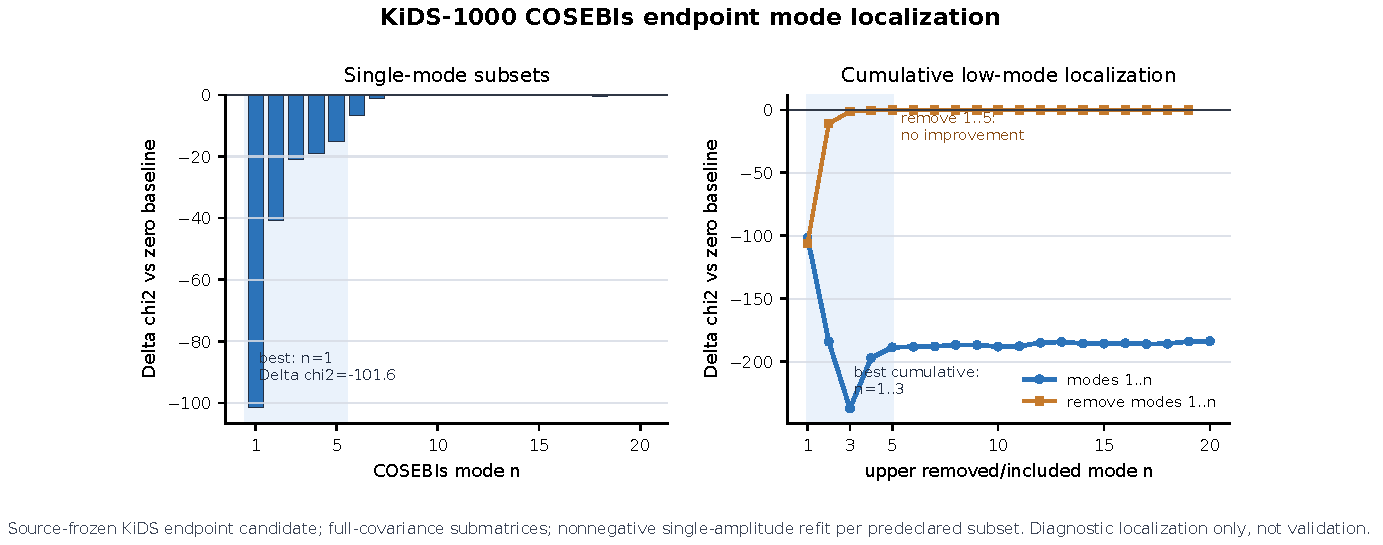
\includegraphics[width=\linewidth]{figures/fig_kids1000_cosebis_mode_localization.pdf}
\caption{KiDS-1000 COSEBIs endpoint mode-localization diagnostic. The left
panel scores single-mode subsets of the source-frozen endpoint candidate. The
right panel compares cumulative low-mode subsets against complementary
low-mode-removal subsets under the same full-covariance submatrix and
nonnegative single-amplitude rule. The improvement is concentrated in the low
COSEBIs modes: \(n=1\) is the strongest single mode, \(n=1\ldots3\) is the
strongest cumulative subset, and removing \(n=1\ldots5\) removes the
improvement. This is a localization diagnostic, not validation.}
\label{fig:kids-mode-localization}
\end{figure}

Because the source-frozen theory shell already contains a deliberately simple,
source-independent mode carrier \(M(n)\propto n^{-1/2}\), we also run a
mode-shape stress audit. The same source-frozen \(W_{\rm path}\) mapping and
the same endpoint scoring rule are kept fixed, but the mode carrier is replaced
by a small predeclared family: flat, \(n^{-0.25}\), the candidate \(n^{-0.5}\),
\(n^{-0.75}\), \(n^{-1}\), \(\sqrt n\), and \(n\). The candidate \(n^{-0.5}\)
carrier remains best in this stress family with
\(\Delta\chi^2=-183.6152665217\). A flat carrier still improves over the zero
baseline, with \(\Delta\chi^2=-136.5504934506\), while the high-\(n\) carrier
gives \(\Delta\chi^2=0\). Thus the low-mode result is carrier-sensitive, but
not reducible in this stress family to the exact \(n^{-1/2}\) choice alone:
low-weighted carriers are preferred, while high-mode weighting removes the
signal. This remains a diagnostic sensitivity result, not validation.

An endpoint-scoring synthesis ledger then aggregates the approved score, the
null-control diagnostics, tomographic-structure robustness, top-control
plausibility audit, jackknife, mode-localization, mode-shape stress, and
physical-promotion blocker ledger. It
computes no new score and claims no validation. Its verdict is that the KiDS
COSEBIs branch contains a low-tail diagnostic endpoint signal, caveated by
tomographic controls and by the physical-promotion blockers. This makes the
next scoring-facing step a predeclared tomographic holdout or an independent
lensing-probe replay, not a physical prediction claim.

We therefore add a separate source-grounding ledger for the low-mode carrier.
It records what is source-side acceptable and what is still open: the
\(n^{-1/2}\) carrier is predeclared, source independent, unit-mean normalized,
retains all \(n=1\ldots20\) modes, and is compatible with a broad coherent
path/readout prior. The mode-localization and mode-shape audits are recorded
only as supporting diagnostics. The ledger verdict is deliberately limited:
partial protocol grounding with an open first-principles mode-kernel derivation
blocker. Thus the carrier is not treated as a final Tau Core lensing theorem.
The next derivation artifact narrows that blocker but does not remove it. If a
smooth path/readout residual carries approximately constant source-side power
per logarithmic COSEBIs mode band, \(dP/d\ln n\simeq\mathrm{const}\), then a
unit-spaced discrete mode bin has \(P_n\propto 1/n\), and the coherent
amplitude envelope satisfies \(M(n)\propto \sqrt{P_n}\propto n^{-1/2}\). The
finite retained mode domain \(n=1\ldots20\) then only fixes the dimensionless
unit-mean normalization. This is a conditional envelope derivation; a covariant
or survey-native lensing path-kernel derivation remains open.
We also add an eligibility gate for using this log-band prior as a protocol
object. The current COSEBIs route passes the ordered-mode-domain,
no-posthoc-mode-cut, source-side path-mapping, and no-high-frequency-only
guardrails. It does not source-prove the smooth coherent path residual
assumption, and it does not close the covariant/survey-native kernel blocker.
Thus the envelope is protocol-eligible for this preflight, but not full-kernel
validated.

As a narrow guardrail, we additionally run a deterministic mock-sanity suite
over the same retained \(15\times20\) COSEBIs row structure. Four synthetic
truth families are compared to four fixed templates: low log-band
\(n^{-1/2}\), flat coherent, high-mode \(n\), and oscillatory alternating. Each
truth recovers its matching template. This is not a physical mock validation and
does not use KiDS data-vector values, fit statistics, random noise, or endpoint
scores. Its role is only to check that the template protocol does not
automatically relabel every deterministic pattern as low-mode.

The final preflight gate in this chain separates survey-native route support
from a full path-kernel derivation. The current route has a source-frozen
mapping basis, a caveated full-route mask-load path proxy, a source-side
path-weight factorization rule, a source-frozen theory-vector shell, and the
deterministic template-recovery guardrail. These items make the route concrete,
but they do not close the kernel derivation. Three blockers remain explicit: a
survey-native operator from path observables to COSEBIs mode response, a
derivation of the log-band prior from that response spectrum, and a covariant
or survey-native lensing/path limit with units and gauge descent audited.
We therefore freeze a narrower mode-response operator specification before any
further scoring: its domain must be a source-side path observable or caveated
path proxy, its codomain is the retained 300-row COSEBIs domain, it must be
linear before endpoint amplitude, it must separate pair/redshift/path support
from mode response, it must use no KiDS data-vector or fit feedback, and it must
have both gauge/mask null safety and a standard-lensing null limit. This is a
specification, not a derivation; the source-native mode-response spectrum and
operator-level null-safety theorem remain open.
We also isolate the spectrum-level part of this missing operator. Under the
explicit smooth coherent path/readout prior, constant power per logarithmic
COSEBIs mode band gives \(P_n\propto 1/n\) and coherent amplitude
\(M_n\propto n^{-1/2}\). This remains conditional: the flat spectrum is kept as
a boundary control, while high-mode and oscillatory spectra are rejected only
under the smooth-path prior. The survey-native response operator and
operator-level gauge/mask null-safety blockers remain open.
We then separate the null-safety blocker into its own operator-level gate. The
available source-frozen null controls have been replayed without endpoint
scores, the retained COSEBIs row domain and caveated path/mask-load proxy are
available, and the uniform web route is retained only as a null control. This
does not prove gauge or mask safety for the future response operator. The gate
therefore leaves three explicit blockers: pure-mask response must be shown to
be quotient-trivial or controlled as a null direction, gauge/coordinate
representation changes must descend to the physical quotient, and the
conditional mode spectrum must be coupled to the null transforms by the same
source-native operator.
The first sub-gate under pure-mask response constructs a source-only mask
perturbation basis rather than a physical response. The full-route
\(F_{\rm overlap}\) and \(D_{\rm path}\) mask observables are centered and
unit-RMS normalized over the 196 route tiles; their centered directions are
non-degenerate, so the resulting pure-mask basis has rank two and can be lifted
to the \(58{,}800\)-row target-by-tile domain. This makes future pure-mask null
replay concrete. It does not prove that those directions are quotient-trivial,
and it does not show that mask-only directions cannot leak into the low-mode
COSEBIs envelope under a future survey-native response operator.
A follow-up source-side leakage audit clarifies this point. Because the
pure-mask directions are centered over route tiles, they collapse to zero under
uniform tile averaging. This is a useful null limit. It is not an operator
theorem: a non-uniform survey-native response could still couple mask-only
tile amplitudes to the same low-mode envelope, so the leakage theorem remains
open.
We therefore add one more source-side gate before treating this branch as an
operator result. The operator-leakage theorem requirements ledger freezes what
a future survey-native theorem must prove: the uniform tile-average null limit
must be recovered, non-uniform mask load must be projected to a quotient-null or
explicit null-control subspace, pure-mask directions must not create a positive
path signal, and the mode spectrum and null descent must be handled by the same
operator. This gate is not a proof. It records two remaining blockers, the
operator leakage theorem itself and gauge/quotient descent, with no use of KiDS
data-vector values, posterior chains, residuals, or endpoint scores.
We also freeze the corresponding gauge/quotient descent requirements. The
future operator must be invariant under admissible representative changes such
as tile relabeling, source-basis recentering, allowed normalization changes,
and pure gauge/null directions. The current source artifacts provide only the
uniform mask-offset null limit and a reproducible route domain. They do not yet
prove normalization invariance, tile-relabeling invariance, pure-mask
control compatibility, or representation independence for a constructed
survey-native operator. The quotient-descent gate therefore remains a blocker,
not a validation claim.
With those blockers made explicit, the repository now records a first
factorized operator-construction attempt. It combines the source-frozen
path/readout mapping component \(M_i\) with the conditional log-band
mode-response weight \(S_n\) into a unit-amplitude skeleton
\[
K_i = M_i S_n .
\]
This is useful because the missing operator is no longer only a name: there is
a reproducible 300-row source-side kernel to audit. It is still not a physical
prediction. The construction does not derive the operator units, does not close
mask leakage, does not prove gauge/quotient descent, and does not use KiDS
data-vector values, posterior chains, residuals, or endpoint scores.
Finally, a physical-units gate separates this source-side skeleton from a
physical COSEBIs readout. The current \(K_i\) is dimensionless and
unit-amplitude. A future result would still need a source-side amplitude map,
the response-unit normalization connecting the kernel to the COSEBIs statistic,
and a standard-lensing/no-\(\tau\)-source null normalization. The covariance
metric can support later scoring, but it is not by itself a derivation of the
operator units.
A source-side amplitude-map attempt then freezes only the internal
dimensionless normalization \(A_{\rm src}=1\) induced by the unit-mean
\(C_{\rm norm}\) rule and the unit-mean operator skeleton. This removes an
arbitrary source-side scale from the skeleton, but it does not derive physical
COSEBIs response units, an endpoint amplitude, or the standard-lensing null
amplitude. The construction uses no KiDS data-vector values, residuals, scores,
posterior chains, or random noise.
A physical-amplitude requirements gate then records the remaining distinction:
\(A_{\rm src}=1\) is an internal dimensionless normalization, whereas a future
physical response amplitude \(A_{\rm phys}\) would still need the missing
COSEBIs response-unit normalization and the standard-lensing/no-\(\tau\)-source
null-amplitude theorem. The covariance metric is kept as a later scoring
metric, but is not treated as an amplitude derivation.
A response-unit normalization requirements gate freezes this first missing
piece more explicitly. The 300-row COSEBIs codomain, the dimensionless
source-side kernel, \(A_{\rm src}=1\), and the covariance metric are available,
but the map that would turn \(A_{\rm src}K_i\) into a physical COSEBIs response
remains open and must be compatible with the standard-lensing null limit.
A standard-lensing null-amplitude theorem-requirements gate then freezes what
that theorem would have to show: source-replayed null controls are only control
limits, the zero-\(\tau\)-source amplitude statement is specified but not
derived, and operator null-safety, gauge/quotient descent, and non-uniform
leakage control remain open blockers.
A final physical-promotion blocker ledger therefore separates diagnostic
endpoint readiness from a physical prediction claim. The diagnostic endpoint
pipeline can be run, but physical promotion remains blocked by five open
requirements: a survey-native operator theorem, an operator leakage theorem,
gauge/quotient descent, response-unit normalization, and the
standard-lensing/no-\(\tau\)-source null-amplitude theorem.

The resulting source-preflight ledger is correspondingly mixed: the 300 COSEBIs
target rows, five-bin redshift-kernel inventory, 196-tile route-coordinate
index, 300-row design skeleton, and 58{,}800-row domain skeleton are available;
the weight-construction rule is source-side computable; the mask shell is only a
partial three-tile source observable; the full path/depth footprint mapping is
represented by a caveated full-route mask-load proxy; the KiDS-footprint
web-environment catalogue remains absent and is therefore represented only by a
uniform null-web control; and null controls have been scored under the approved
endpoint run. Thus the lensing branch is now narrowed to a source-side ready,
geometry-audited, endpoint-scored but not validated protocol rather than an
unspecified missing-input state.

The null-control gate is declared in parallel. It predeclares sky rotation,
tomographic-pair shuffle, wrong-channel activation, and web/path sign-flip
control families. A future endpoint must freeze the control seed and
multiplicity policies before any null score is interpreted.
The present package now freezes that seed/multiplicity layer as a protocol
artifact: deterministic seeds and fixed planned multiplicities are recorded for
the four control families, totaling 1008 control draws. These controls are then
replayed against the source-frozen unit-amplitude theory-vector shell and saved
only as deterministic vector digests and source-side summary statistics. No
control score is computed, no likelihood replay is executed, and no KiDS data-vector value or
residual is used to choose the seeds or multiplicities.

Finally, the repository includes a tiny pilot product-freeze manifest in the
source-manifest data folder. It hash-locks three public distance-side files: a
cosmic-chronometer \(H(z)\) table, a Pantheon+ distance table, and a Pantheon+
STAT+SYS covariance matrix. These are provenance and covariance-shape tests,
not endpoint inputs. The Pantheon+ table and covariance dimensions are checked
during reproduction. All pilot rows keep the endpoint permission flag set to
false, because the associated mask, calibration, nuisance-parameter, and
systematics policies are not yet frozen.

The first endpoint-eligible distance scope is also frozen without scoring. For
Pantheon+, the residual-blind row rule is to exclude Cepheid calibrators and
retain rows with \(z_{\rm HD}\ge 0.023\). This yields 1371 retained rows out of
1701 source rows, with the full STAT+SYS covariance dimension checked against
the source table. The resulting row mask is a source-derived artifact only:
no \(\Lambda\)CDM residuals, Tau residual parameters, fit-improvement flags, or
late-time activation fits are used.

The first scoring grammar is then frozen as a protocol artifact. The declared
baseline family is a flat-\(\Lambda\)CDM distance modulus branch with analytic
marginalization of the absolute magnitude/Hubble offset. The declared Tau
comparison family is only the late-activation shell
\(W_\tau(a)=a^q/(a^q+a_\tau^q)\). The required controls include baseline-only,
Tau-shell, shuffled-activation, and wrong-activation branches.

As a final dry-run layer, the repository builds a Pantheon+ design matrix with
1371 rows. It contains source columns, the scale factor \(a=1/(1+z_{\rm HD})\),
and fixed activation-family basis columns. It deliberately excludes model
predictions, residuals, likelihoods, \(\chi^2\) values, fit-improvement flags,
and fitted Tau parameters. This verifies that the frozen scope and scoring
grammar can produce numerical inputs without crossing into endpoint scoring.

The repository also includes the first numerical Pantheon+ pilot scoring run,
marked throughout as \(\texttt{PILOT\_SCORING\_NOT\_VALIDATION}\). This run is
a diagonal-covariance smoke test of the frozen scoring grammar, not a
covariance-complete cosmological likelihood. It uses the diagonal of the
retained STAT+SYS covariance submatrix, analytic intercept marginalization, and
the frozen grid declared in the pilot manifest. On this grid the Tau
late-activation shell has a slightly lower diagonal-covariance \(\chi^2\) than
the flat-\(\Lambda\)CDM branch,
\[
\Delta\chi^2_{\tau-\Lambda{\rm CDM}}=-0.084,
\]
but its AIC is worse,
\[
\Delta{\rm AIC}_{\tau-\Lambda{\rm CDM}}=+5.916,
\]
because the shell carries more effective parameters. This is therefore a
pipeline and claim-boundary test, not evidence for dark energy, not validation
of Tau Core cosmology, and not a replacement for a full-covariance analysis.

The next pilot layer repeats the same frozen branch grammar with the retained
Pantheon+ STAT+SYS covariance submatrix, using Cholesky solves and no
eigenvalue-floor regularization. This full-covariance run is marked as
\(\texttt{FULL\_COV\_PILOT\_SCORING\_NOT\_VALIDATION}\). On the same 1371-row
scope, the Tau late-activation shell again has a slightly lower
\(\chi^2\) than the flat-\(\Lambda\)CDM branch,
\[
\Delta\chi^2_{\tau-\Lambda{\rm CDM}}=-0.192,
\]
but again loses under AIC,
\[
\Delta{\rm AIC}_{\tau-\Lambda{\rm CDM}}=+5.808.
\]
Thus the full-covariance pilot preserves the same interpretation as the
diagonal smoke test: the scoring pipeline is operational, but the present
single-probe evidence is weak and model-selection negative for the Tau shell.
This should be read primarily as a limitation of the homogeneous late-activation
shell, not as a true negative against the broader Tau Core
morphology/projection-readout framework. In particular, the pilot tests only a
single isotropic activation family \(W_\tau(a)\). It does not yet contain the
multi-channel morphology, observer/path, or time/readout projection structure
suggested by the broader Tau Core readout framework.

A subsequent low-redshift source-basis refinement makes this limitation more
explicit. The first void/source-basis attempts and the caveated partial
\(W_{\rm path}\) route are retained as diagnostic attempts rather than as
validation claims. Simple coupled path--void/web variants and a bank of
monotone path transforms improve the baseline only weakly and do not survive
their frozen controls. A broader path/sky/environment screen is also globally
non-positive: its best overall candidate is not control-resistant. However, one
narrow family, \(W_{\rm path}\times\mathrm{sky}_z\), survives its own
predeclared family controls. After a separate external permission-only review,
the repository replays only this family on the same 12-row partial path scope.
The replay gives
\[
  \Delta\chi^2_{\mathrm{sky}_z-\Lambda{\rm CDM}}=-0.44407920978,
  \qquad
  \Delta\chi^2_{\mathrm{sky}_z-{\rm best\ control}}=-0.06205941383,
\]
with zero family controls beating the candidate. This is the best
control-surviving result among the current low-redshift source-basis
experiments, and it points toward observer/path projection as the most
promising channel tested so far. It remains a 12-object, permission-only
diagnostic replay, not population validation and not a physical
lensing-path-weight derivation.  A subsequent source-side refinement tests a
centered observer-orientation kernel,
\[
  K_{v2}=W_{\rm path}\left(\mathrm{sky}_z-\langle \mathrm{sky}_z\rangle_{\rm scope}\right),
\]
under a separate permission-only authorization.  This centered kernel improves
the baseline,
\[
  \Delta\chi^2_{v2-\Lambda{\rm CDM}}=-0.47326976306,
\]
but does not survive its predeclared controls: one deterministic-shuffle
control is slightly better
\[
  \Delta\chi^2_{v2-{\rm best\ control}}=+0.01875086453.
\]
Thus the centered observer-orientation replay is recorded as a diagnostic
negative, not as a new positive replay.  It suggests that the raw narrow
\(W_{\rm path}\times\mathrm{sky}_z\) signal is not trivially strengthened by
subtracting the scope monopole; a better source-side observer/projection basis
is needed before any broader claim.  A subsequent accelerated source-side
observer-basis bank therefore tests predeclared sky-vector and redshift-centered
basis functions before any new replay claim.  Its strongest family is
\[
  W_{\rm path}\times \mathrm{sky}_x\times z_{\rm centered},
\]
which is then sent through a separate reviewer authorization and replayed only
after the reviewer returns
\texttt{GO\_OBSERVER\_BASIS\_REPLAY\_PERMISSION\_ONLY}.  The resulting
permission-only replay gives
\[
  \Delta\chi^2_{\rm obsbasis-\Lambda CDM}=-0.58072431813,\qquad
  \Delta\chi^2_{\rm obsbasis-best\ control}=-0.08783266799,
\]
with rank one among the candidate and frozen controls and zero controls better
than the candidate.  This is the strongest current narrow observer/projection
signal in the low-redshift sequence, but it is still a 12-object diagnostic
replay rather than population validation.  It should also be read as a
deliberately simplified kernel, not as the full Tau Core observer/path
projection.  The replayed factor
\(W_{\rm path}\times\mathrm{sky}_x\times z_{\rm centered}\) keeps only a
source-frozen path proxy, one Cartesian sky-direction component, and a
scope-centered redshift coordinate.  A full observer/path kernel would have to
replace this low-dimensional proxy by a source-grounded function of the full
sky direction, redshift, line-of-sight environment, void/web geometry, survey
and observer-frame orientation, metric/lensing-path information, and possible
time/readout phase variables.  The present result therefore motivates a
full-kernel construction; it does not supply one.

As a first check of this limitation, we also ran a preauthorization
full-kernel-proxy screen that multiplies the same observer-basis carrier by
already frozen source-side void, web, line-of-sight environment, and
void-geometry proxies.  This screen is not a replay authorization and is not
validation.  Its best family remains the simpler
\(W_{\rm path}\times\mathrm{sky}_x\times z_{\rm centered}\), with
\(\Delta\chi^2=-0.58072431813\) relative to flat \(\Lambda\)CDM.  The best
global control in the enlarged proxy bank is slightly better than this best
candidate by \(\Delta\chi^2=0.115454\), and only two families survive their
own local controls.  The only surviving enriched family is weaker:
\[
W_{\rm path}\times\mathrm{sky}_x\times z_{\rm centered}
\times W_{\rm web,centered}\times \rho_{\rm los,centered},
\]
with \(\Delta\chi^2=-0.451413\) relative to flat \(\Lambda\)CDM and
\(\Delta\chi^2=-0.048323\) relative to its best local control.  We therefore
record the enlarged proxy-bank result as a diagnostic constraint: adding
available source-side void/web/environment multipliers does not automatically
improve the observer-basis signal.  A genuine full observer/path kernel will
need stronger source-side grounding, not merely additional proxy factors.
A component audit makes this constraint explicit.  No enriched proxy family is
stronger than the base observer-basis carrier.  The mixed void--web factor is
close to the base carrier but fails its sign/control test; the mixed
web--line-of-sight-density factor survives its local controls but remains
weaker than the base carrier.  Pure line-of-sight, void-geometry, void, and web
single-factor extensions are weak or control-failed.  This pattern is useful
because it prevents over-reading the observer/projection result: the current
evidence favours a narrow source-grounded observer-basis direction, not
arbitrary accumulation of available environmental proxies.
Accordingly, the next full-kernel gate is now source-observable rather than
score-observable: a future replay must first freeze a full observer-frame basis,
a radial line-of-sight environment integral, path-aware void geometry,
directional web anisotropy, independent metric/lensing-path information, and
independent time/readout phase evidence.  Until such observables are frozen, the
present kernel remains a reduced observer/path proxy.
We have begun this source-observable step for the line-of-sight environment by
constructing a residual-blind radial shell profile from the same SDSS DR17 MCPM
source catalogue.  The profile uses five predeclared redshift shells
(foreground far, foreground near, near-source, background near, background far)
inside the same 2 degree cone.  It provides complete five-shell support for
153 of the 424 low-redshift rows, and for 7 of the 12 partial path-scope rows
(10 of those 12 have at least one non-empty shell).  This is progress toward a
path/environment observable, but it is not yet a full line-of-sight path
integral: coverage is incomplete and no metric, lensing, or null-geodesic
bundle weighting has been derived.
We also construct a source-side path-aware void-geometry observable.  Instead
of using only the nearest void to the source position, this artifact computes
the closest approach of each VoidFinder void center to the observer--source
segment, records the impact parameter and the phase along the segment, and
flags effective-radius crossings.  In the current low-redshift sample, 180 of
424 rows have an effective-void path crossing; in the 12-object partial
path-scope replay set, 10 rows have such a crossing.  This partially satisfies
the void-geometry requirement of the future full kernel, but remains a low-z
Euclidean path proxy rather than a metric/lensing-weighted null-geodesic bundle
term.
We next construct the first R4 source-side directional web-anisotropy
observable.  Using the same SDSS DR17 MCPM source catalogue, we freeze a
2 degree cone and a redshift window of \([-0.03,+0.03]\) around each low-z
Pantheon+ source, then compute tangent-plane density-weighted dipole and
quadrupole moments of the local web support.  This makes the web channel
directional rather than purely scalar: 238 of 424 low-redshift rows are
quadrupole-ready, and 9 of the 12 partial path-scope rows are quadrupole-ready.
This is still not a full web tensor contracted with a metric/lensing-weighted
observer--source path, and it does not authorize endpoint replay.  It is a
partial source observable for a future full observer/path kernel.
The R5 metric/lensing-path route audit is also made explicit.  Public KiDS and
CMB lensing routes are cached, and the low-redshift Pantheon+ rows are
cross-checked against the KiDS DR4.1 tile-coordinate inventory.  Only 5 of 424
low-redshift rows are within 1 degree of a KiDS tile proxy, and no
source-aligned convergence, shear, mass-map integral, or metric/lensing path
weight is computed.  Thus R5 is route-grounded but not yet
observable-grounded; it remains a blocker for any physical path-weight claim.
The first concrete CMB-lensing source-product acquisition route is then frozen
through the public NASA LAMBDA ACT DR6 lensing release.  The manifest records
the provider information page, provider download script, expected byte count,
local byte count, checksum when available, and the endpoint-disabled claim
boundary.  This strengthens data availability for R5, but it is still only
source-side acquisition: no HEALPix convergence map is synthesized from the ACT
alm product, no convergence or shear value is sampled at Pantheon+ rows, and no
metric/lensing-weighted null-geodesic path integral is constructed.  Therefore
the ACT DR6 acquisition route does not by itself authorize observer/path
endpoint replay.  The accompanying source inventory records 13 ACT DR6 lensing
variants with kappa alm, mask, filter, and noise products; the baseline variant
is available as the recommended science route, while the difference-map and curl
variants provide source-native null-control routes for a future sampling gate.
Finally, we update the R6 time/readout source audit.  The cosmic-chronometer
\(H(z)\) table is fetched and frozen, the SDSS DR16 multi-tracer BAO/RSD
products are fetched and frozen, and the Planck/LAMBDA CMB route page is
cached.  Under the present coverage rule, all 424 low-redshift Pantheon+ rows
have nearby CC \(H(z)\) redshift support.  However, no \(\Delta_{\rm clock}\),
\(\Delta_{\rm clock,\ast}\), redshift-bin phase rule, or numeric \(W_{\rm time}\)
activation is derived or frozen.  R6 is therefore route-grounded but still
activation-blocked.
As a narrow follow-up subgate, we freeze only a source-side normalization
candidate,
\[
\Delta_{\rm clock,\ast}^{\rm cand}
  = {\rm median}\left(\sigma_H/H\right)_{\rm CC}
  = 0.16581626506,
\]
computed from the fetched/frozen cosmic-chronometer table.  This is not a
time/readout residual and not a \(W_{\rm time}\) activation.  It only removes
one source-side scale ambiguity; the actual \(\Delta_{\rm clock}\) observable,
redshift-bin phase rule, and numeric \(W_{\rm time}\) rule remain future work.
We also freeze a source-side redshift-bin policy candidate.  Each low-redshift
Pantheon+ row is assigned to the source-native cosmic-chronometer support cell
defined by the midpoints to adjacent CC \(H(z)\) nodes; the SDSS BAO/RSD
redshift nodes are recorded only as route markers.  This fixes the
source-side domain on which a future \(\Delta_{\rm clock}\) observable could be
evaluated, but it does not smooth \(H(z)\), compute \(\Delta_{\rm clock}\), or
activate \(W_{\rm time}\).
Finally, as a source-side uncertainty-channel candidate, we define
\[
\Delta_{\rm clock}^{\rm unc}
  =
  \log\left[
    \frac{(\sigma_H/H)_{\rm assigned\ CC\ bin}}
         {{\rm median}(\sigma_H/H)_{\rm CC}}
  \right].
\]
This quantity is dimensionless and residual-blind.  It should be read only as
a CC measurement-uncertainty/readout contrast, not as a physical clock-drift
measurement.  In the present low-redshift support assignment it spans
\([0.0476000829881,\,0.834341816646]\).  A numeric \(W_{\rm time}\) activation
rule is still not frozen.
As a final source-side preprocessing step, we freeze a candidate basis
\[
W_{\rm time}^{\rm unc}
  =
  \frac{\Delta_{\rm clock}^{\rm unc}
        - \langle\Delta_{\rm clock}^{\rm unc}\rangle_{\rm source}}
       {\sigma_{\rm source}(\Delta_{\rm clock}^{\rm unc})}.
\]
This basis spans \([-4.23048519997,\,2.81443932804]\) and has zero source mean.
It is not an endpoint replay and not a validation claim; it is only a
source-side candidate that would require a separate authorization/control gate
before entering scoring.
That gate is represented by a replay-authorization review package whose full
checksum is recorded in the released package summary.  The package is not
completed in the present draft and does not authorize endpoint replay.
After completion of the external authorization response, we run the single
permission-only replay.  The result is diagnostic: the candidate basis improves
slightly over the baseline
\((\Delta\chi^2_{\rm cand-baseline}=-0.652452012)\), but it is not
control-resistant.  Three controls outperform the candidate, with
\texttt{rank\_reverse} the best control.  We therefore retain this branch as evidence
that a simple CC-uncertainty time/readout basis is insufficient by itself, not
as validation of a time/readout channel.
This negative diagnostic is also structurally informative.  In Tau Core
language the time/readout projection is not expected, in its full form, to be a
homogeneous function of redshift or scale factor alone.  It should be treated
as potentially observer/path dependent and morphology aware: the effective
clock readout may depend on the source environment, large-scale void/web
structure, the null-geodesic bundle reaching the observer, and the local
readout phase by which \(a(t)\), \(H(t)\), distances, and metric observables are
extracted from the deeper configuration.  The tested
\(W_{\rm time}^{\rm unc}\) basis is therefore only a deliberately narrow
source-side stress test.  Its control failure motivates a richer source-frozen
\(W_{\rm time}\) basis rather than a stronger claim about time projection.
We also record a first preauthorization overlap screen between the current
observer-basis carrier and this narrow time/readout basis on the same 12-row
observer scope.  The screened source-frozen families are the pure observer
carrier, the \(W_{\rm time}^{\rm unc}\) basis restricted to the observer scope,
a multiplicative observer--time coupling, and an additive observer--time proxy.
The best family remains the pure observer carrier,
\[
  W_{\rm path}\times\mathrm{sky}_x\times z_{\rm centered},
  \qquad
  \Delta\chi^2=-0.58072431813,
\]
while the best multiplicative observer--time coupling is weaker
\((\Delta\chi^2=-0.477935)\), the additive proxy is weaker
\((\Delta\chi^2=-0.423746)\), and the time basis alone is nearly inactive on
this scope \((\Delta\chi^2=-0.030493)\).  This screen is not a replay
authorization and not validation.  Its function is diagnostic: the present
CC-uncertainty \(W_{\rm time}\) proxy does not improve the already successful
narrow observer/path proxy when the two are combined.  A future combined
observer--time kernel should therefore be built from a better source-native
clock/readout observable, not by reusing this uncertainty basis as if it were a
physical time-projection channel.
We then replace the uncertainty-only basis by a more direct source-side
clock-rate/phase candidate from the same fetched cosmic-chronometer table.  For
each low-redshift Pantheon+ row, the assigned CC support bin defines a
source-normalized \( \log H(z) \) level, a finite-difference
\(d\log H/d\log(1+z)\) slope, and a normalized product basis.  This is still a
coarse low-redshift candidate because the present low-\(z\) sample occupies
only three CC support bins; it is not a physical clock-drift measurement and
does not authorize replay.  A preauthorization fast screen gives the best
candidate in the product phase family, with
\[
  \Delta\chi^2_{\rm phase-\Lambda CDM}=-0.523771964.
\]
However, the family is again not control-resistant: the best global control is
a rank-reversed clock-level control with \(\chi^2=377.625521\), well below the
candidate \(\chi^2=381.270425\).  We therefore record the clock-rate/phase
branch as a useful negative diagnostic.  Direct CC rate information is more
physically relevant than the uncertainty-only basis, but the current
low-redshift binning is too coarse and too vulnerable to redshift-ordering
controls to support a time/readout replay claim.
A follow-up rank-control audit localizes the failure mode.  The low-redshift
sample occupies only three CC support bins, with row counts \(397\), \(20\),
and \(7\), and each clock family has at most three unique basis values.  The
rank-reversed control is the best local control for all three clock families.
Thus the blocker is not merely that the candidate is weak; the present clock
proxy is too coarse and rank-control dominated to be endpoint-ready.  This is a
negative source-side diagnostic, not evidence against a more complete
observer/path-dependent time/readout projection.

We therefore run one narrower follow-up stress test: keep the same CC source
table, but widen the support from the low-\(z\) subset to all Pantheon+ rows
covered by the CC redshift range.  This includes \(1370/1371\) retained
Pantheon+ rows, uses 31 nearest-neighbor CC support cells, and excludes one row
above the CC support.  The best candidate shifts to the clock-slope family and
improves the baseline by
\[
  \Delta\chi^2_{\rm slope-\Lambda CDM}=-1.142872.
\]
Moreover, this clock-slope family survives its own local controls.  However,
the global control gate still fails: a rank-reversed clock-level control has
\(\chi^2=1207.578076\), while the best clock-slope candidate has
\(\chi^2=1208.99638\).  We therefore record the CC-support run as a more
promising but still non-replay diagnostic.  It narrows the viable
time/readout direction toward a source-justified clock-slope route, but it does
not yet establish a control-resistant Tau Core \(W_{\rm time}\) kernel.
We freeze this as a route gate rather than as an endpoint.  The route status is
\[
  \texttt{CLOCK\_SLOPE\_REVIEW\_CANDIDATE\_ENDPOINT\_BLOCKED\_BY\_GLOBAL\_CONTROL}.
\]
The allowed next step is a reviewer-gated clock-slope-only candidate.  The
source-side reason is that the slope tracks a rate of expansion readout,
\(d\log H/d\log(1+z)\), whereas the clock-level branch is closer to a
background-level control and the phase product remains a mixed diagnostic.
Endpoint replay or validation language remains forbidden until the global
rank-control blocker is resolved.
Accordingly, we prepare a reviewer authorization package for a possible
permission-only clock-slope route.  The package is not completed and contains
no endpoint residuals, endpoint scores, or fit statistics.  Its purpose is only
to ask whether a later clock-slope-only replay candidate may be prepared while
the global rank-control blocker remains explicitly acknowledged.

As an independent source-side route audit, we also inspect the frozen SDSS
multi-tracer BAO/RSD products for a non-CC time/readout observable.  The radial
BAO entries obey
\[
  D_H/r_d = c/(H(z)r_d),
\]
so \(-\log(D_H/r_d)\) is proportional to \(\log H(z)\) up to the unresolved
sound-horizon nuisance \(r_d\).  The audit finds exactly two usable radial BAO
rows, at \(z_{\rm eff}=0.700\) and \(0.845\).  This route is independent of
Pantheon distance residuals and independent of the CC clock-level route, but it
is underresolved and does not solve the \(r_d\) nuisance.  We therefore record
it only as source-side route discovery:
\[
  \texttt{independent\_radial\_bao\_time\_observable\_present\_but\_underresolved\_not\_replay}.
\]
It does not authorize replay and does not validate a Tau Core time/readout
kernel.
We then run a joint CC+BAO consistency audit using only source-side quantities:
the two radial BAO points and the nearest CC support values.  This audit is
useful precisely because it prevents an overclaim.  In the current two-point
comparison, radial BAO aligns with the CC \(\log H\) level route
(\(\texttt{bao\_cc\_level\_two\_point\_alignment}=1\)) and anti-aligns with the
CC clock-slope route
(\(\texttt{bao\_cc\_slope\_two\_point\_alignment}=-1\)).  Thus radial BAO
currently supports an independent expansion-level time/readout observable, not
the current CC clock-slope route.  The machine-readable verdict records this
as a BAO-level alignment, a non-slope alignment, and an underresolved non-replay
status.  The resulting synthesis is therefore deliberately conservative: a
clock-slope review candidate plus an independent, underresolved BAO-level
route, not an endpoint.
The allowed next route is either completion of the external clock-slope
authorization package or construction of separate source-side level/slope time
routes that still contain no endpoint scores.  Endpoint replay, validation
language, and any claim that radial BAO already supports the clock-slope route
remain forbidden until a joint nuisance/interface policy is frozen and the
current blockers are closed.
We therefore freeze a route-split ledger with two non-endpoint branches.  The
`time-level' branch records independent BAO support and CC-level alignment, but
keeps the two-point and \(r_d\)-nuisance blockers.  The `time-slope' branch
records the CC clock-slope candidate signal, but keeps the global-control and
reviewer-authorization blockers and explicitly forbids using radial BAO as
clock-slope support.  This split is a bookkeeping result, not a new endpoint
score.
For the time-level branch we also freeze a nuisance/interface plan.  Since the
source observable is \(D_H/r_d\), the current use is restricted to two-point
directional level alignment.  The plan forbids fitting \(r_d\) from Pantheon
residuals, claiming an absolute \(H(z)\) scale without an \(r_d\) policy, or
using radial BAO as clock-slope support.  Before endpoint scoring, a future
source gate must freeze either an external \(r_d\) prior or an \(r_d\)
marginalization policy and expand the radial-BAO support.
As a first safe use of the level branch, we also run a differential audit.  In
the two-point difference,
\[
  \Delta[-\log(D_H/r_d)] = \Delta[\log H],
\]
the constant \(r_d\) term cancels.  The resulting source-side check has the
same sign as the nearest-CC \(\log H\) difference, but the BAO differential
signal is very low significance
(\(\texttt{delta\_bao\_snr}=0.0997626410319\)).  We therefore record this only
as a directional route-discipline result, not as amplitude evidence, endpoint
replay, or validation.
The associated \(r_d\)-policy selection gate therefore accepts only the
`\(r_d\)-cancelled differential direction' policy for current source-side use.
An external \(r_d\) prior and analytic \(r_d\)-marginalization are recorded as
future routes pending source/protocol freeze, while fitting \(r_d\) from
Pantheon residuals is explicitly forbidden.
The external-prior route now has a source-side freeze protocol and blank
response template.  It accepts only independently sourced prior families such as
Planck-2018 base-\(\Lambda\)CDM \(r_{\rm drag}\), DESI/BAO external priors, or
BBN+BAO external priors, with explicit fields for value, uncertainty,
assumption family, source reference, URL/DOI, extraction note, and source hash
or page cache.  The current state is protocol-ready but numeric-prior-empty:
no external \(r_d\) value is yet frozen and no endpoint replay is opened.
We then freeze a first caveated external-prior response from Planck 2018
base-\(\Lambda\)CDM TT,TE,EE+lowE+lensing, using the published Table~2
\(r_{\rm drag}\) value \(r_d=147.09\pm0.26\,{\rm Mpc}\).  This is an
early-universe nuisance prior for a future time-level route only.  It uses no
Pantheon residuals, endpoint scores, or late-time fit parameters, and it does
not authorize endpoint replay.
We also freeze the analytic nuisance interface for an absolute radial-BAO
level route.  Since
\[
  -\log(D_H/r_d)=\log H+\beta_{r_d},\qquad
  \beta_{r_d}:=\log r_d-\log c ,
\]
in consistent units, \(\beta_{r_d}\) is treated as a source-side nuisance
parameter rather than as a Tau Core signal.  The allowed future handling is
only analytic linear nuisance projection or a predeclared \(r_d\)-prior
marginalization.  The protocol forbids Pantheon residuals, endpoint scores,
late-time fit parameters, posthoc \(r_d\) choices, and any claim that radial
BAO supports the clock-slope route.
We further declare the required future endpoint-control suite before any
time-level replay: \(r_d\)-off, external-prior-width stress, wrong-prior,
BAO-pair-drop, CC-match-window, level/slope-swap, and redshift-order-shuffle
controls.  This is only a control-family declaration; the controls are not
replayed here and a future seed manifest remains required before endpoint
interpretation.
Finally, we declare the allowed BAO-support expansion routes before importing
any additional radial BAO values: public DESI radial BAO products,
eBOSS/SDSS LyA-QSO radial BAO, and an independent low-redshift BAO
cross-check compilation.  This expansion manifest imports no new values and
opens no replay; it only states that a future time-level endpoint should have
at least four independent radial BAO support bins under source-frozen
provenance.
As the first concrete source-freeze step on that path, we cache and hash-lock
the public DESI DR2 combined Gaussian BAO mean/covariance files distributed
through the DESI/Cobaya public BAO likelihood
route~\cite{DESIDR2BAO2025,DESIDR2Products2025}.  The frozen DESI inventory
contains 13 BAO rows, including six radial \(D_H/r_d\) rows, and a 13 by 13
covariance block.  This is not a replay result: the DESI rows are not yet
inserted into the time-level design matrix, \(r_d\)-marginalization interface,
or endpoint-control suite.
We then freeze the radial time-level interface itself by converting the six
DESI \(D_H/r_d\) rows into \(y=-\log(D_H/r_d)=\log H+\beta_{r_d}\) and
propagating the radial covariance subblock with the Jacobian
\(C_{y,ij}=C_{x,ij}/(x_i x_j)\).  This still leaves \(\beta_{r_d}\) as a
nuisance parameter and does not match the DESI rows to cosmic-chronometer
support.
The first chronometer-support ledger then matches the DESI radial rows to the
nearest frozen cosmic-chronometer \(H(z)\) support without smoothing or
extrapolation.  Five of the six DESI radial rows lie within the chronometer
redshift range; the \(z=2.33\) Ly-\(\alpha\) row is explicitly marked as
outside chronometer coverage rather than extrapolated.
The corresponding readiness gate closes only source-side blockers: the external
\(r_d\) source freeze, the joint \(r_d\)-marginalization definition, the
endpoint-control-suite definition, the BAO expansion manifest, and the DESI DR2
source-inventory, radial-interface, chronometer-match ledger, high-redshift row
policy, and deterministic control-seed freezes.  The high-redshift \(z=2.33\)
Ly-\(\alpha\) row is predeclared as excluded from the first chronometer-matched
endpoint and retained as high-\(z\) holdout or future independent-clock support.
The first DESI/chronometer endpoint scope is therefore five radial rows, with
seven frozen control families and deterministic seeds \(41001\)--\(41007\).  The
time-level endpoint remains blocked because no endpoint authorization/replay
review has been completed.  The older two-point SDSS-only BAO difference remains
recorded as a low-significance diagnostic, but is not treated as an active
blocker for the DESI route.
The machine-readable ledger therefore records that source support and controls
are frozen, while endpoint replay remains unauthorized.
A separate reviewer handoff package has therefore been prepared for this final
authorization step.  The package contains the frozen scope, source ledgers,
control seeds, and a blank reviewer-response template; it contains no endpoint
residuals, endpoint scores, or fit statistics, and all replay/validation flags
remain false until a completed authorization response is validated.
The corresponding replay-run grammar is also frozen as a template: it fixes the
five allowed DESI radial rows, the excluded high-\(z\) row, the seven control
families, and the forbidden inputs, while keeping
\({\tt endpoint\_replay\_allowed=false}\).
The completed external authorization response has now been imported and
validated with decision
\({\tt GO\_DESI\_CC\_5ROW\_TIME\_LEVEL\_REPLAY\_PERMISSION\_ONLY}\).  This
authorizes preparation of one guarded replay under the frozen scope and
controls, but still does not produce an endpoint score and keeps both endpoint
validation and physical-validation claims false.
The guarded replay has now been executed as a permission-only diagnostic.  It
fits the constant \(\beta_{r_d}\) nuisance over the five DESI/chronometer rows
and obtains \(\chi^2=5.5243\), but the candidate does not survive the frozen
controls: the deterministic redshift-order shuffle control gives
\(\chi^2=2.1455\).  The replay verdict is non-control-resistant and
non-validating. This negative control result is retained as part of the audit
trail.
A focused diagnostic of this failure mode shows that the five-row constant-level
endpoint is ordering-fragile rather than physically decisive: the candidate has
\(\chi^2/{\rm dof}=1.3811\), while the deterministic redshift-order shuffle has
\(\chi^2/{\rm dof}=0.5364\), and four frozen controls beat the candidate in
\(\chi^2\).  The largest candidate diagonal pull is at \(z_{\rm eff}=1.321\).
The diagnostic failure mode is that the five-row constant-\(\beta_{r_d}\)
endpoint is ordering-fragile.
This is not a reason to tune the candidate post hoc; it is a reason to require
richer independent clock support or a more informative time/readout observable
before a DESI time-level endpoint claim.
We therefore freeze a negative-control response gate. It keeps replay disabled
and allows only a source-side time/readout expansion manifest as the next
action. The expansion manifest records five requirements before any future DESI
time-level replay can be considered: high-\(z\) independent clock support,
multiple independent clock supports or explicit caveats for each BAO row, a
source-frozen time/readout shape observable beyond a constant level, preserved
ordering and leave-row controls, and a joint covariance/nuisance policy. Its
current endpoint-ready route count is zero; the next primary source gate is
high-\(z\) independent clock support, with a time/readout shape observable as a
parallel route.
The first high-\(z\) support audit has now been run. The frozen
cosmic-chronometer table contains 32 rows and ends at \(z=1.965\), while the
excluded DESI Ly-\(\alpha\) radial row is at \(z=2.33\). Its nearest frozen
clock support is therefore \(\Delta z=0.365\) away, and the target is not
bracketed without extrapolation. The verdict is that the high-\(z\) row remains
a holdout; it cannot enter a replay until an independent high-\(z\) clock or
time/readout route is source-frozen.
In parallel, we freeze a source-side time/readout shape observable that removes
the constant \(\beta_{r_d}\) nuisance rather than fitting another level.  The
observable uses adjacent first differences of
\(-\log(D_H/r_d)-\log H_{\rm CC}\) over the five CC-matched DESI rows, together
with an uneven-grid second-difference curvature proxy.  It yields four
first-difference rows and three curvature rows, with maximum diagonal
signal-to-noise values \(1.9032\) and \(1.7232\), respectively.  This is useful
because it identifies a frozen candidate shape for future time/readout work, but
it remains below endpoint status: it still uses only the five nearest-neighbor
chronometer matches, and the high-\(z\) Ly-\(\alpha\) row remains unsupported by
an independent clock route.  The recorded verdict is therefore
\({\tt desi\_time\_readout\_shape\_candidate\_frozen\_but\_not\_endpoint\_ready}\).
We also map this frozen shape observable onto the current Tau Core general
readout-basis language.  In that ledger, the adjacent-difference clock-slope
and curvature shapes are classified as \(K_{\rm time}\) candidates, radial BAO
level information remains \(K_{\rm closure}\) context rather than clock
support, and redshift-order controls are retained as \(K_{\rm null}\).  This
mapping does not complete projection induction: activation is source-candidate
only, quotient survival is not proven against the ordering null, closure
stability remains partial, and 4D readout survival is not endpoint-authorized.
The recorded claim boundary is therefore
\({\tt time\_shape\_maps\_to\_K\_time\_candidate\_but\_projection\_induction\_incomplete}\),
not a time-projection validation claim.
We also freeze the corresponding \(K_{\rm null}\) ordering-control suite.  A
future shape-route replay must preserve five controls:
redshift-order shuffle, leave-row or leave-pair sensitivity, CC-window stress,
wrong-time-basis controls, and \(r_d\)-prior or marginalization stress.  At the
present stage only the redshift-order shuffle is already available from the
negative-control diagnostic, and no control is yet bound to the shape route.
The suite verdict is
\({\tt k\_null\_ordering\_controls\_declared\_but\_not\_shape\_bound}\), so the
quotient-survival gate remains open.
A first shape-bound control-vector ledger then binds these controls without
endpoint scores or endpoint residuals.  Redshift-order shuffle is bound as a
shuffled first-difference source vector; leave-row sensitivity is bound as
leave-shape-row masks; wrong-time-basis controls are bound through curvature and
rank-reverse shape vectors; and the \(r_d\)-prior stress is an analytic null
because first differences remove a constant \(\beta_{r_d}\).  The remaining
CC-window stress is now bound through the Row4 source-side review chain as a
caveated source-window control.  This closes the unbound-control bookkeeping
gap, but it does not authorize replay because the CC-window control is
caveated and a separate replay authorization is still absent.
A separate multi-clock support audit makes this limitation more concrete.  It
checks whether each of the five authorized radial rows has at least two clock
entries and at least two independent reference sources in fixed redshift
windows.  Three of five rows pass a strict \(\Delta z\le 0.05\) window. Four of
five pass a relaxed \(\Delta z\le 0.10\) window, but radial row 4 remains
blocked because the two relaxed-window clock entries come from only one
independent reference source.  The route is therefore still not endpoint-ready:
the shape observable exists, but independent clock redundancy is incomplete.
We therefore prepare an independent shape-review handoff rather than a replay
authorization.  The package asks only whether the adjacent-difference/curvature
observable may be retained as a caveated source-side diagnostic candidate. It is
blank, uncompleted, contains no endpoint residuals, endpoint scores, or fit
statistics, and keeps endpoint replay disabled.
Its completed-response validator accepts only a non-replay outcome that retains
the shape as a caveated source-side candidate; without such an external response,
the route status remains unchanged.
A separate replay-authorization handoff is then prepared after the five
shape-route controls have been bound.  This second package asks only whether
the already frozen DESI shape route may advance to replay. It is still blank
and uncompleted, contains no endpoint residuals, endpoint scores, or fit
statistics, records five bound controls with no unbound control family, and
keeps endpoint replay disabled until a completed external authorization response
is validated.  Its claim boundary is replay authorization review, not endpoint
validation.  The completed-response validator can only convert a reviewer
approval into permission-only replay status; it still requires validation and
physical-validation flags to remain false, and rejects any response that uses
forbidden endpoint fields.
The completed external response gives
\({\tt GO\_DESI\_SHAPE\_ROUTE\_REPLAY\_PERMISSION\_ONLY}\). This authorizes
one separate predeclared DESI shape-route replay, but it does not claim endpoint
validation or physical validation.
The corresponding replay-run template freezes the same five-row radial scope,
four adjacent shape rows, three curvature rows, and five shape-bound control
families. It remains authorization-required and keeps endpoint replay disabled;
it is a run grammar, not a replay result.
With that authorization in place, the permission-only shape-route replay reports
a source-native quadratic shape score of \(5.52425578108\) for the frozen
\({\tt CLOCK\_SLOPE\_SHAPE}\) candidate. The strongest frozen control is the
leave-shape-row control with score \(5.50939872844\), so the candidate exceeds
all controls but only by a narrow margin of \(0.01485705264\). We therefore
record this as a positive permission-only replay signal with weak
control-margin, not as endpoint validation or physical validation.
An internal robustness stress preserves this claim boundary. The candidate
remains ranked first by the frozen shape score, but the fractional margin over
the strongest control is only \(0.00268942156713\), and the strongest
leave-one-row stress retains \(0.997310578432\) of the full candidate score.
The stress verdict is therefore
\({\tt positive\_but\_narrow\_margin\_and\_row\_sensitive\_not\_validation}\):
the replay signal survives the frozen controls, but the DESI shape route is
still narrow-margin and row-sensitive.
The row-ablation view gives the more useful interpretation.  Dropping shape row
2, the row later isolated as the most source-caveated middle row, leaves a
score of \(4.13850507326\), or \(0.749151602906\) of the full candidate score.
Thus row 2 is important, but not the sole carrier of the shape-route signal.
By contrast, dropping row 1 leaves only \(0.669168123641\) of the score, making
row 1 the most required row in this diagnostic, while dropping row 0 leaves
\(0.997310578432\) and is nearly dispensable.  The claim-safe conclusion is
therefore pattern-level rather than single-row: the DESI shape-route replay is
not explained by row 2 alone, but the positive route-wide signal remains
narrow-margin and source-sensitive.
Table~\ref{tab:desi-shape-route-robustness} records the stress in compact
form. The table is deliberately interpreted as an internal robustness ledger,
not as a validation table.

\begin{table}[t]
\centering
\caption{DESI shape-route permission replay and internal robustness stress.
All rows keep \texttt{endpoint\_validation\_claimed=false} and
\texttt{physical\_validation\_claimed=false}.}
\label{tab:desi-shape-route-robustness}
\footnotesize
\begin{tabular}{p{0.28\linewidth}p{0.22\linewidth}p{0.42\linewidth}}
\toprule
Quantity & Value & Claim-safe reading\\
\midrule
Frozen candidate score & \(5.52425578108\) & Candidate
\({\tt CLOCK\_SLOPE\_SHAPE}\) is rank \(1\) by the frozen quadratic shape
score\\
Best frozen control score & \(5.50939872844\) & Strongest control is the
leave-shape-row stress; the candidate-control margin is only
\(0.01485705264\)\\
Fractional margin & \(0.00268942156713\) & Positive but narrow-margin replay
signal\\
Strongest leave-one stress & \(0.997310578432\) of candidate & Row-sensitive;
one dropped-row stress nearly reproduces the full candidate score\\
Drop Row2 stress & \(0.749151602906\) of candidate & Row2 alone is not the
full signal carrier; the route-level pattern mostly survives without it\\
Most required row & Row1; \(0.669168123641\) retained when dropped & Middle
shape rows carry the core signal; Row1 is the strongest row-sensitivity point\\
Strongest leave-two stress & \(0.83195519127\) of candidate & The signal is not
purely single-row, but it is not yet broad validation evidence\\
Verdict & positive, narrow, row-sensitive & Permission-only replay evidence,
not endpoint or physical validation\\
\bottomrule
\end{tabular}
\end{table}

\begin{figure}[t]
\centering
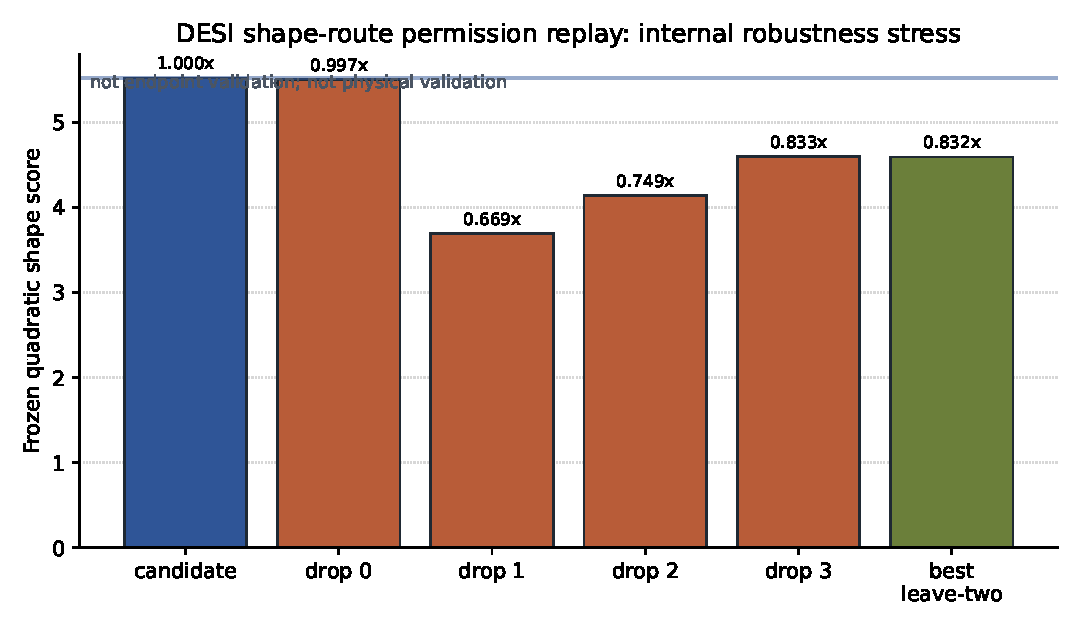
\includegraphics[width=0.82\linewidth]{figures/fig_desi_shape_route_robustness_stress.pdf}
\caption{DESI shape-route robustness stress generated from the frozen replay
artifact. The candidate remains first, but the strongest leave-one-row stress
nearly reproduces the full candidate score. The figure is an internal
permission-replay diagnostic, not endpoint validation.}
\label{fig:desi-shape-route-robustness}
\end{figure}
A follow-up row-sensitivity source audit then maps the same stress result back
onto the frozen DESI/CC source rows. It finds that shape row 0 is the most
dispensable row, while the middle rows 1 and 2 form the core-sensitive part of
the signal. Row 1 spans the \(z=0.706\) to \(z=0.934\) interval and is supported
by different current CC reference families in the manifest. Row 2 spans
\(z=0.934\) to \(z=1.321\), but both endpoints currently come from the same
reference family, so it remains source-caveated. The resulting status is
that the middle shape rows carry the core signal, but one of them is still
source-caveated; the machine-readable verdict is recorded in the source-audit
CSV.
The next concrete source-side action is therefore independent clock or shape
support for rows 1 and 2, especially row 2, before any promotion of the DESI
shape route.
A dedicated shape-core acquisition manifest freezes this into a narrow work
order: \({\tt DESI\_SHAPE\_ROW\_2\_CORE\_SUPPORT}\) is the \(P0\) target because
it is core-sensitive and single-reference caveated, while
\({\tt DESI\_SHAPE\_ROW\_1\_CORE\_SUPPORT}\) is the \(P1\) confirmatory target
because row 1 is the most required row. This manifest does not fetch sources,
does not authorize replay, and does not claim validation.
A scan of the already frozen cosmic-chronometer table then finds one existing
independent in-interval support point for the \(P0\) row-2 target:
Moresco et al.~\cite{Moresco2012ExpansionRate} at \(z=1.037\), with
\(H(z)=153.7\pm19.6736\) km s\(^{-1}\) Mpc\(^{-1}\). This partially strengthens
row 2, because it supplies non-Simon clock support inside the same
\(z=0.934\)--\(1.321\) interval. It is not, however, a full endpoint-pair
replacement and does not make the DESI shape route endpoint-ready.
For the \(P1\) row-1 target, the same frozen CC scan supplies two independent
in-interval confirmatory support rows, Borghi et al. at \(z=0.75\) and Stern
et al. at \(z=0.88\).  These are attached as source-side confirmation for the
most required row, but they likewise do not create an endpoint-ready status and
do not authorize replay.
A repository-independent Row1 source-review package was prepared for exactly
this narrow question.  The completed reviewer response accepts the Borghi and
Stern rows as confirmatory independent in-interval Row1 support, while
explicitly keeping endpoint replay, endpoint validation, physical validation,
and route promotion false.
The Row2 Moresco point is therefore attached only as a reviewed source-side
support ledger:
the source key is \({\tt Moresco2012ExpansionRate}\), the attachment verdict is
\({\tt row2\_moresco2012\_in\_interval\_support\_attached\_partial\_not\_endpoint\_ready}\),
and the replay and validation flags remain false. In other words, the row-2
source caveat is reduced, but the route still requires endpoint-pair
independence or external review before any promotion.
A repository-independent source-review package is prepared for exactly this
question. It asks whether the Moresco (2012) attachment may be accepted as
caveat-reducing in-interval support, and it explicitly forbids endpoint replay,
endpoint validation, physical validation, and endpoint-pair replacement.
The completed reviewer response accepts the attachment only in that narrow
source-side sense. The machine verdict is
\({\tt row2\_moresco2012\_attachment\_accepted\_as\_caveat\_reducing\_not\_endpoint\_ready}\);
all replay and validation flags remain false. Thus row 2 is better supported
than before, but the DESI shape route still requires endpoint-pair independence
or a separate replay/promotion gate before any stronger status can be claimed.
A promotion-readiness ledger then freezes this exact status:
\({\tt row2\_caveat\_reduced\_but\_endpoint\_pair\_independence\_blocker\_remains}\).
Consequently, row 2 is strengthened but
\({\tt row2\_promotion\_ready=false}\), and the shape route is not promoted by
this source-side review.
We then run a focused endpoint-pair independence scout against the already
frozen cosmic-chronometer table.  The scout finds one strict independent
right-endpoint candidate, Moresco (2015), but no strict independent
left-endpoint support.  Its machine verdict is
\({\tt row2\_endpoint\_pair\_independence\_not\_satisfied\_in\_frozen\_CC\_table}\).
Thus the Moresco (2012) attachment remains a caveat reducer rather than an
endpoint-pair replacement: row 2 is still not promotion-ready, and the next
source-side task is independent left-endpoint clock support or a source-native
shape-support route before any replay or promotion is considered.
The left-endpoint near-miss freeze makes the remaining blocker more precise:
two independent relaxed-window candidates exist, Stern et al. (2010) at
\(z=0.88\) and Moresco et al. (2012) at \(z=0.8754\).  The closest candidate
misses the frozen strict endpoint window only narrowly,
\(|0.88-0.934|=0.054\) for a strict window of \(0.05\), but it is still outside
the predeclared gate.  The machine verdict is
\({\tt row2\_left\_endpoint\_has\_relaxed\_independent\_nearmisses\_but\_no\_strict\_support}\).
This motivates a separate source-window review or a source-native shape-support
search; it does not release the left endpoint and does not authorize replay.
A repository-independent source-window review package is therefore prepared for
exactly this question.  It is intentionally blank and asks only whether the
relaxed near-miss sources may be retained as caveated source-window context.  It
contains no endpoint residuals, endpoint scores, or fit statistics, and it keeps
\({\tt left\_endpoint\_release\_allowed=false}\),
\({\tt row2\_promotion\_ready=false}\), and replay disabled until a completed
response is separately validated.
The completed-response validator is deliberately conservative: even the
strongest allowed positive response can only record
\({\tt source\_reopen\_caveated=true}\).  It still keeps
\({\tt left\_endpoint\_release\_allowed=false}\),
\({\tt row2\_promotion\_ready=false}\), and all replay/validation flags false;
any completed response that attempts to set replay or validation flags is
rejected before canonical artifacts are modified.
The companion decision gate resolves the current machine state.  Since no
completed response has been imported it would record pending status.  The
completed reviewer response is now imported and validates the strongest allowed
source-side outcome:
\({\tt ROW2\_LEFT\_SOURCE\_REOPEN\_CAVEATED\_NO\_REPLAY}\), with verdict
\({\tt row2\_left\_source\_reopen\_caveated\_no\_replay}\).  This reopens the
left-endpoint route only as caveated source context.  It still keeps
\({\tt left\_endpoint\_release\_allowed=false}\),
\({\tt row2\_promotion\_ready=false}\),
\({\tt shape\_route\_promotion\_allowed=false}\), and all replay/validation
flags false.
The post-window-review source plan then freezes the only allowed next source
targets.  Its status is
\({\tt ROW2\_SOURCE\_REOPENED\_CAVEATED\_LEFT\_ENDPOINT\_STILL\_NOT\_RELEASED}\):
the source route is reopened only in a caveated source-side sense, with strict
left-endpoint support still at zero.  The two P0 targets are independent strict
left-endpoint support inside the frozen window, or source-native shape support
for the row-2 interval.  Both routes explicitly forbid endpoint residuals,
endpoint scores, and kernel-performance feedback.
The left strict-support scout preserves the current negative source-side
result.  In the frozen cosmic-chronometer table the nearest point to the row-2
left endpoint is the existing same-family Simon et al. (2005) point at
\(z=0.9\); the nearest independent candidate is Stern et al. (2010) at
\(z=0.88\), with \(|\Delta z|=0.054\), just outside the strict \(0.05\)
window.  The verdict is
\({\tt row2\_left\_strict\_support\_absent\_in\_frozen\_cc\_table}\).  Thus
the strict-left P0 route remains genuinely open and no replay or promotion is
authorized.
The complementary source-native shape-support scout finds that the row-2
interval does have DESI DR2 BAO shape information at both endpoints:
\({\rm DM}/r_s\) and \({\rm DH}/r_s\) at \(z=0.934\) and \(z=1.321\), with a
positive-definite covariance subblock.  It freezes the source-native vector
\(\Delta\log({\rm DM}/r_s)=0.246281910984\),
\(\Delta\log({\rm DH}/r_s)=-0.218701863111\), and
\(\Delta\log[({\rm DM}/{\rm DH})]=0.464983774095\).  This is positive
source-side support for the shape route, but it still uses no endpoint residuals
or scores and keeps \({\tt row2\_promotion\_ready=false}\).
The corresponding external review package is built as a blank source-side-only
package.  It asks whether this DESI DR2 source-native BAO vector may be accepted
as caveat-reducing row-2 support.  It contains the frozen source rows,
covariance source files, inventory, scout artifacts, and response template, but
no endpoint residuals, endpoint scores, or fit statistics.  Its package verdict
is
\({\tt row2\_source\_native\_shape\_support\_review\_package\_ready\_not\_completed}\).
The completed external response accepts the vector as caveat-reducing
source-native shape context:
\({\tt row2\_source\_native\_shape\_support\_accepted\_as\_caveat\_reducing\_not\_endpoint\_ready}\).
This reduces the row-2 source caveat, but it does not make Row2 endpoint-ready,
does not promote the route, and does not authorize replay.
The Row2 gate-status ledger freezes the combined state as
\({\tt ROW2\_ENDPOINT\_REPLAY\_BLOCKED\_PROMOTION\_NOT\_READY}\):
the source-native shape context has passed review and both source-side caveats
are reduced, but Row2 remains non-promotion-ready and endpoint replay remains
forbidden.
The follow-up Row2 promotion-review package is therefore only a handoff asking
whether a separate future replay-authorization package may be prepared.  It is
not replay authorization, not endpoint validation, and not a route-success
claim.
The completed promotion-review response accepts only this narrow handoff:
\({\tt row2\_promotion\_review\_accepts\_preparing\_separate\_replay\_authorization\_not\_direct\_replay}\).
The Row2 gate-status ledger is therefore updated to
\({\tt ROW2\_SEPARATE\_REPLAY\_AUTH\_REVIEW\_ALLOWED\_NOT\_REPLAY}\).
This still keeps \({\tt endpoint\_replay\_allowed=false}\); it only allows a
separate replay-authorization package to be prepared.  That package is now built
as a permission-only reviewer handoff asking whether one frozen Row2 replay may
later be run.  It contains no endpoint residuals, endpoint scores, or fit
statistics, and it does not authorize validation or physical interpretation.
The completed replay-authorization response accepts this narrow scope with the
verdict
\({\tt GO\_DESI\_SHAPE\_ROW2\_REPLAY\_PERMISSION\_ONLY}\).  The ledger therefore
records
\({\tt ROW2\_PERMISSION\_ONLY\_REPLAY\_AUTHORIZED\_NOT\_VALIDATION}\):
\({\tt endpoint\_replay\_allowed=true}\) only for one frozen Row2 diagnostic
replay, while \({\tt endpoint\_validation\_claimed=false}\),
\({\tt physical\_validation\_claimed=false}\), and
\({\tt shape\_route\_promotion\_allowed=false}\) remain fixed.
The authorized Row2-only replay has now been run as an isolated diagnostic.  It
does not survive the local controls:
\({\tt row2\_permission\_replay\_candidate\_not\_control\_resistant\_not\_validation}\).
The frozen candidate score is \(0.415519707291\), while the strongest local
control, \({\tt control\_redshift\_order\_shuffle\_ROW2}\), scores
\(1.62654904473\).  This negative local result is retained: it says that Row2
alone does not carry the full DESI shape-route signal, not that the full route
is validated or falsified.
Combined with the route-wide ablation result above, this is a useful negative
control rather than a hidden failure: Row2 is locally weak, yet the route-wide
candidate retains about \(75\%\) of its score when Row2 is removed.  The current
interpretation is therefore that the shape-route evidence is a multi-row
pattern with a narrow control margin, not a Row2-only effect.
A final shape-core support synthesis gate freezes this interpretation in one
non-scoring ledger.  It combines the route-wide robustness stress, the
row-sensitivity audit, the core source-support scan, the Row2 source-side
reviews, and the isolated Row2 permission replay.  Its status is
\({\tt DESI\_SHAPE\_CORE\_SUPPORT\_SYNTHESIS\_BUILT\_SOURCE\_STRENGTHENED\_NOT\_VALIDATION}\).
The gate records rows 1 and 2 as the core rows, Row1 as the most required row,
with confirmatory independent source support externally accepted, and Row2 as
caveat-reduced but not promotion-ready.  It also records the Row2 permission
replay as negative against local controls.  Thus the allowed reading is
source-side strengthening of a multi-row, narrow-margin shape-route signal, not
endpoint validation, not physical validation, and not falsification.
The current reproducibility replay preserves exactly this boundary.  Re-running
the frozen full shape-route permission replay gives the same candidate score
\(5.52425578108\), the same strongest control score \(5.50939872844\), and the
same narrow margin \(0.01485705264\).  The replay therefore remains positive in
the permission-only sense, but the synthesis gate keeps
\({\tt endpoint\_replay\_allowed\_by\_this\_gate=false}\).  The next allowed
scientific step is not another stronger replay claim, but a route-level
source-synthesis review that asks whether the Row1 and Row2 source-side support
is jointly sufficient to motivate any later validation-oriented gate.
That reviewer handoff is now prepared as a repository-independent package.  It
contains the policy, response template, synthesis-gate ledger, Row1 source
review response, Row2 source-side review responses, and the isolated Row2
diagnostic context.  Its checksum is
\({\tt a7c71dc3d5e9d5adeb3ce3313177dba0f757d80465b3e3834ff4c48ddd4f56f9}\).
The package status is
\({\tt DESI\_SHAPE\_ROUTE\_SOURCE\_SYNTHESIS\_REVIEW\_PACKAGE\_BUILT\_NOT\_COMPLETED}\).
It is a source-side review handoff only: the response template keeps
\({\tt endpoint\_replay\_allowed=false}\),
\({\tt endpoint\_validation\_claimed=false}\),
\({\tt physical\_validation\_claimed=false}\), and
\({\tt shape\_route\_promotion\_allowed=false}\).  A completed response may at
most support preparation of a future separate gate; it cannot by itself
authorize replay or validation.
The completed source-synthesis response accepts exactly this limited reading:
\({\tt ACCEPT\_AS\_SOURCE\_SYNTHESIS\_SUPPORT\_FOR\_FUTURE\_GATE\_PREPARATION\_NOT\_REPLAY\_NOT\_VALIDATION}\).
All four review questions are accepted, with
\({\tt forbidden\_inputs\_used=false}\).  The response records
\({\tt future\_gate\_preparation\_allowed=true}\), but keeps
\({\tt shape\_route\_promotion\_allowed=false}\),
\({\tt endpoint\_replay\_allowed=false}\),
\({\tt endpoint\_validation\_claimed=false}\), and
\({\tt physical\_validation\_claimed=false}\).  The practical consequence is
therefore narrow: the source state is strong enough to prepare a separate
authorization gate, but the present paper still treats the DESI shape route as
a source-strengthened, narrow-margin diagnostic rather than validation.
A post-synthesis gate-authorization package is therefore prepared as the next
handoff.  Its role is only to ask whether a later replay-authorization package
may be prepared under the accepted source-synthesis state.  The package checksum
is
\({\tt 4a125b1cc20e54d93de131e68c6798ae6ec2de74030abf5855d590ad190aecfd}\).
It explicitly preserves the narrow-margin replay status
\((0.01485705264)\), the row-sensitive robustness verdict, and the rule that no
current replay, endpoint validation, physical validation, or route promotion is
authorized.  Thus the gate sequence is deliberately staged: source synthesis
may motivate preparing a later authorization package, but the present package
does not itself open that replay.
The completed post-synthesis gate response accepts this preparation step with
\({\tt ACCEPT\_PREPARE\_SEPARATE\_VALIDATION\_ORIENTED\_GATE\_PACKAGE\_NOT\_REPLAY\_NOT\_VALIDATION}\).
It sets \({\tt prepare\_later\_authorization\_package\_allowed=true}\), while
keeping \({\tt endpoint\_replay\_allowed=false}\),
\({\tt endpoint\_validation\_claimed=false}\), and
\({\tt physical\_validation\_claimed=false}\).  This changes only the project
workflow: a separate validation-oriented gate package may now be prepared, but
the current DESI shape-route result is still not promoted to validation.
That separate gate package is now built as a blank reviewer handoff.  It asks
whether a future completed response may authorize one frozen permission-only
DESI shape-route replay diagnostic under the caveat-aware scope.  Its checksum
is
\({\tt 26fddf67c46cd82585ecc185abee13e0c309ba8c9c3c6b657b4d8d4bcbf8ec52}\).
The package itself still keeps \({\tt endpoint\_replay\_allowed=false}\),
\({\tt endpoint\_validation\_claimed=false}\), and
\({\tt physical\_validation\_claimed=false}\).  A future completed response
would therefore be required before any new replay can be run.
The completed validation-oriented gate response is now imported with decision
\({\tt GO\_DESI\_SHAPE\_VALIDATION\_ORIENTED\_PERMISSION\_REPLAY\_ONLY}\).
This accepts preparation for a future permission-only diagnostic replay, but it
still keeps
\({\tt endpoint\_replay\_allowed=false}\),
\({\tt endpoint\_validation\_claimed=false}\),
\({\tt physical\_validation\_claimed=false}\), and
\({\tt forbidden\_inputs\_used=false}\).  It also explicitly retains the
narrow-margin caveat, the row-sensitive robustness caveat, and the Row2
negative-diagnostic caveat.  Consequently the scientific status is unchanged:
the shape route is worth a later permission-only diagnostic authorization, but a
separate completed replay-authorization response is required before any new run.
That final permission-only replay authorization package is now prepared as a
blank reviewer handoff with checksum
\({\tt 03dd33a4968f710adf0490fe9d8e9e1e2c4298455202aab4af795905dbb3579d}\).
It asks only whether one future frozen DESI shape-route permission-only
diagnostic replay may be authorized.  The package itself still keeps
\({\tt endpoint\_replay\_allowed=false}\),
\({\tt endpoint\_validation\_claimed=false}\), and
\({\tt physical\_validation\_claimed=false}\) until a completed reviewer
response is validated.
The completed validation-permission authorization response then accepts exactly
one frozen permission-only diagnostic replay with decision
\({\tt GO\_DESI\_SHAPE\_VALIDATION\_PERMISSION\_REPLAY\_ONLY}\), while
retaining \({\tt endpoint\_validation\_claimed=false}\),
\({\tt physical\_validation\_claimed=false}\), the narrow-margin caveat, the
row-sensitive caveat, and the Row2 negative-diagnostic caveat.  That replay has
now been run as a separate artifact.  The candidate score is
\({\tt 5.52425578108}\), the best frozen control is
\({\tt control\_leave\_shape\_row\_max}\) with score
\({\tt 5.50939872844}\), and the margin is
\({\tt 0.01485705264}\).  Thus the candidate remains ahead of all frozen
controls, but only by a narrow, row-sensitive margin.  The recorded verdict is
\({\tt desi\_shape\_validation\_permission\_replay\_candidate\_exceeds\_all\_controls\_not\_validation}\).
Finally, the DESI clock-support acquisition manifest freezes the two concrete
missing source targets before any further source search.  The first is radial row
4 at \(z_{\rm eff}=1.484\), where relaxed-window clock support exists but comes
from only one independent reference family.  The second is the excluded
high-\(z\) row at \(z_{\rm eff}=2.33\), which requires independent clock or
time-readout support that covers or brackets the row without extrapolation.  The
manifest is not a data fetch, not a replay authorization, and not a validation
claim; it only makes the next acquisition step narrow and auditable.
The first candidate scan does not close either gate. The VANDELS chronometer
measurement at \(z=1.26\)~\cite{Tomasetti2023VANDELS}, the LEGA-C chronometer
measurement at \(z=0.8\)~\cite{Jiao2023LEGAC}, and the photometric chronometer
proof-of-principle at \(z=0.75\)~\cite{Jimenez2023PhotometricCC} are useful
source-side context, but they do not provide independent support in the frozen
\(z=1.484\) row-4 window.  The eBOSS DR16 QSO BAO/RSD route is close to row 4
at \(z_{\rm eff}=1.48\)~\cite{Hou2020QSOBAORSD}, but it is a clustering
measurement, not a second independent clock-reference family.  The eBOSS/SDSS
Ly-\(\alpha\) BAO route at
\(z=2.33\)~\cite{duMasdesBourboux2020LyA,SDSSLyAForestVAC} does cover the
high-\(z\) row, but it is a BAO/\(r_d\) cross-probe route rather than an
independent clock measurement.  It is therefore retained only as a
cross-probe/control context, not as high-\(z\) clock support.
The route is consequently closed as an active source-side blocker rather than
advanced to replay: a future DESI time-readout attempt must first freeze either
an independent row-4 clock reference near \(z=1.484\), or an independent
high-\(z\) clock/source-native time-readout route covering \(z=2.33\) without
extrapolation.
A completed external source-side review partially reopens only the row-4 source
acquisition gate: the reviewer identified independent cosmic-chronometer entries
bracketing \(z=1.484\), namely \(z=1.43\) and \(z=1.53\) in the chronometer
compilation summarized by Moresco~\cite{Moresco2023ChronometersReview}.  This
does not authorize replay.  The high-\(z\) row at \(z=2.33\) remains blocked,
and BAO/RSD plus Ly-\(\alpha\) BAO remain cross-probe context unless independent
clock or source-native time-readout evidence is attached.
Freezing the source-native values sharpens the conclusion: the bracket entries
are \(H(1.43)=177\pm18\) and \(H(1.53)=140\pm14\)
km s\(^{-1}\) Mpc\(^{-1}\), both attributed to Simon, Verde, and
Jimenez~\cite{Simon2005Chronometers}.  They improve the explicit row-4 source
record, but because they reuse the Simon et al. reference family they do not
release the original independent-reference-family blocker.  Row 4 therefore
remains outside replay until non-Simon independent clock or source-native
time-readout support is frozen.
We therefore run a stricter non-Simon row-4 source search under the frozen
\(|\Delta z|\le 0.10\) window.  The closest non-Simon chronometer source
currently attached to this chain is the Moresco (2015) measurement at
\(z=1.363\), \(H(z)=160\pm33.6\) km s\(^{-1}\) Mpc\(^{-1}\)
~\cite{Moresco2015RaisingBar}.  This is an independent reference family, but
\(|1.363-1.484|=0.121\), outside the frozen row-4 window.  The strict-window
search is therefore negative: it records useful near-miss context, but no
row-4 replay release, no endpoint claim, and no validation claim.
We therefore prepare a separate row-4 source-window review handoff, asking only
whether the strict window should remain fixed or whether the Moresco (2015)
near miss may be retained as caveated source-side context.  That handoff is not
a replay authorization and contains no endpoint residuals, scores, or fit
statistics.
The completed source-blocker review accepts this near-window source only in the
weak sense allowed by the protocol: row 4 may be reopened for caveated
source-side acquisition, with the strict \(|\Delta z|\le0.10\) window retained
as the default and with no endpoint replay, validation claim, or physical claim.
In parallel, we freeze a separate row-5 high-\(z\) source-review handoff for the
excluded \(z_{\rm eff}=2.33\) Ly-\(\alpha\) row.  This handoff asks whether a
public, citable high-\(z\) clock/chronometer source, or a source-native
time/readout observable, can support the row without treating Ly-\(\alpha\) BAO
alone as clock support.  Its validator allows a positive reviewer response only
as source-side reopening or as a request for a separate replay-authorization
review; it keeps row-5 endpoint replay disabled.  A corresponding row-5
decision gate resolves the state into
\({\tt ROW5\_HIGH\_Z\_REVIEW\_PENDING\_NOT\_REPLAY}\),
\({\tt ROW5\_HIGH\_Z\_BLOCKER\_REMAINS\_NOT\_REPLAY}\), or source-reopen
status, but never into endpoint validation.
The completed row-5 review finds no independent high-\(z\) clock or
source-native time/readout observable covering \(z=2.33\); Ly-\(\alpha\) BAO is
therefore retained as cross-probe context only.
A focused Row-5 source-route scout reaches the same conclusion with updated
context.  DESI DR1 cosmic chronometers provide new direct measurements at
\(z=0.46,0.67,\) and \(0.83\)~\cite{Loubser2025DESICC}, strengthening the DESI
clock-source family but not bracketing the \(z=2.33\) row.  The current
cosmic-chronometer review/forecast literature likewise frames percent-level
future chronometer improvements as possible but does not supply a frozen
\(z=2.33\) clock value for this route~\cite{Moresco2024CosmicChronometers}.
Thus the high-\(z\) row remains a holdout or future source-native time/readout
target rather than a replay input.
The post-review holdout confirmation gate makes this consequence explicit:
radial row 5 remains excluded from the first CC-matched endpoint scope
\((0,1,2,3,4)\), not because it was removed after scoring, but because no
source-side gate-closing high-\(z\) clock/readout source has been frozen.
A post-review priority ledger therefore changes the next DESI time-route task:
the primary gate is no longer high-\(z\) row inclusion, but derivation of a
source-frozen time/readout shape observable beyond the constant
\(\beta_{r_d}\) level, with ordering controls preserved.
The route-level closure ledger consequently records the DESI time-readout
branch as closed pending source blockers: row 4 is caveated source-reopened but
not replay-ready, row 5 remains high-\(z\) clock blocked, the negative-control
response gate still blocks replay, and replay remains disabled until richer
clock/readout support is source-frozen and a separate replay-authorization
handoff exists.

\begin{figure}[t]
\centering
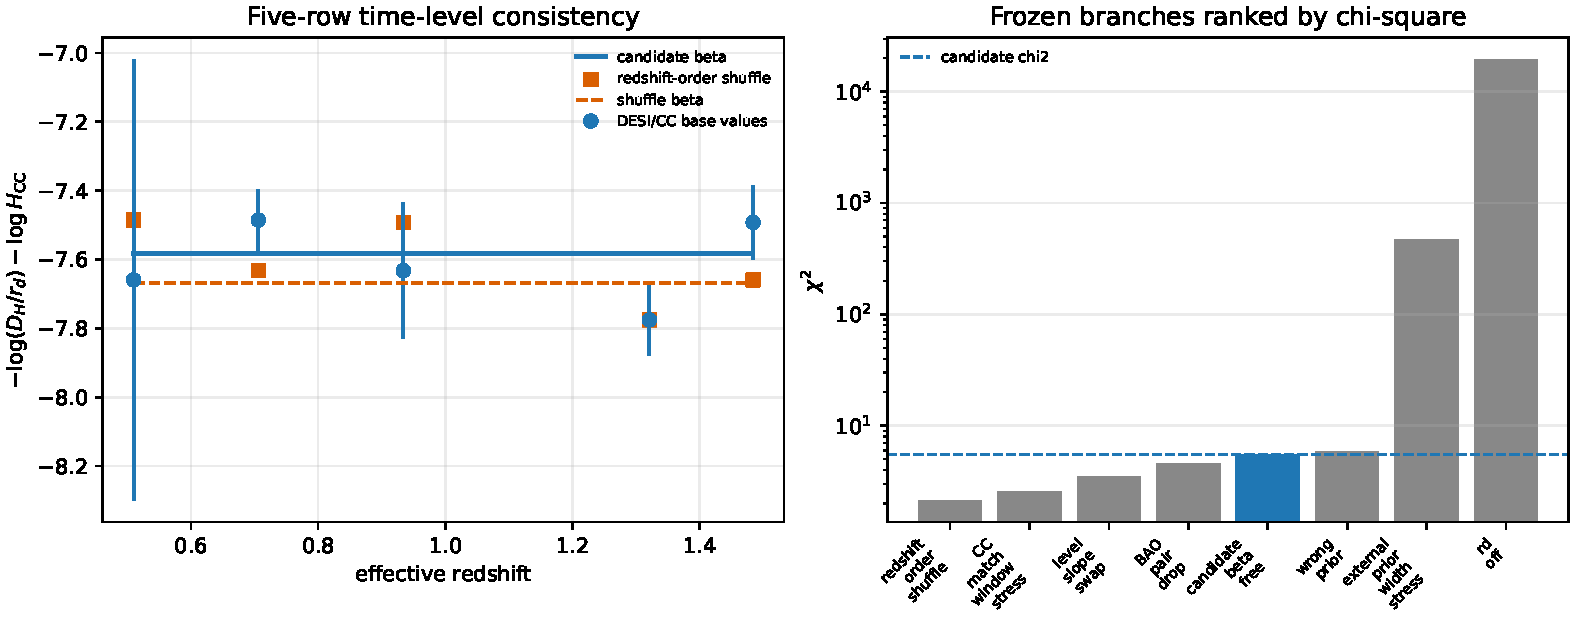
\includegraphics[width=\linewidth]{figures/fig_desi_time_level_negative_control_diagnostic.pdf}
\caption{DESI/chronometer time-level negative-control diagnostic. The left
panel shows the five frozen values of
\(-\log(D_H/r_d)-\log H_{\rm CC}\) with the fitted constant nuisance level
\(\beta_{r_d}\), together with the deterministic redshift-order shuffle control.
The right panel ranks the frozen replay branches by \(\chi^2\) on a logarithmic
scale. The candidate is not numerically pathological, but it is not
control-resistant: several frozen controls, especially the redshift-order
shuffle, fit the five-row constant-level test better. This figure is a
negative-control diagnostic, not endpoint validation.}
\label{fig:desi-time-negative-control}
\end{figure}

\begin{figure}[t]
\centering
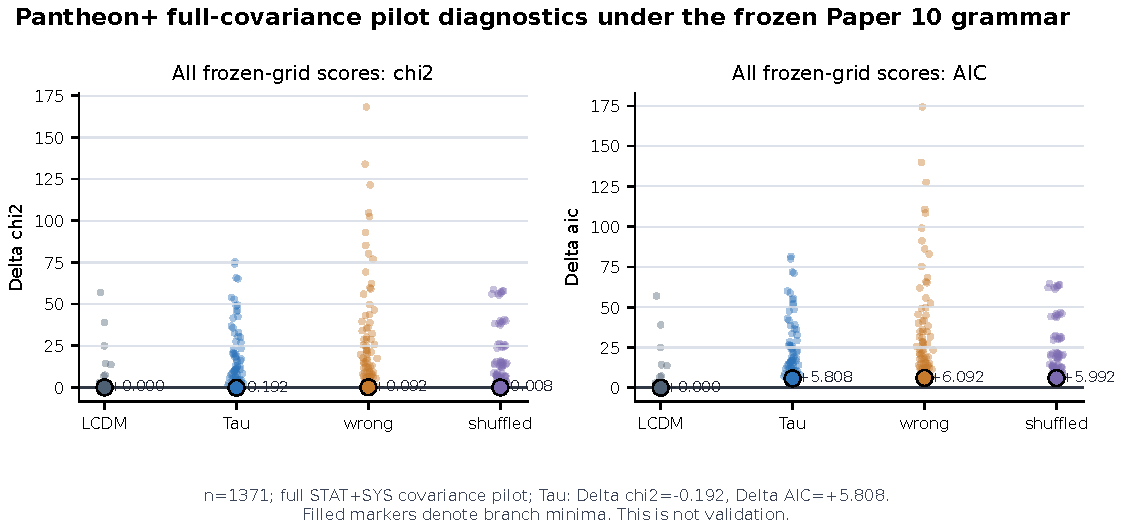
\includegraphics[width=\linewidth]{figures/fig_pantheon_full_cov_pilot_branch_diagnostics.pdf}
\caption{Pantheon+ full-covariance pilot scoring diagnostics under the frozen
Paper 10 grammar.
Each panel shows all finite grid scores relative to the best
flat-\(\Lambda\)CDM branch. The x-axis labels denote flat-\(\Lambda\)CDM,
Tau-shell, wrong-activation, and deterministic shuffled-activation branches;
filled markers denote branch minima. The Tau shell obtains a tiny
full-covariance \(\chi^2\) improvement but loses under AIC, so the figure should
be read as a scoring-pipeline diagnostic, not as cosmological validation.}
\label{fig:pantheon-pilot-diagnostics}
\end{figure}

\section{Numeric joint-ledger gate}

After the channel-level \(z_i\) distribution ledger was built, a separate
reviewer authorization package was prepared for the only allowed next
operation: combining the already frozen \(z_i\) values under the already frozen
symbolic shell \(T_{\rm joint}=\sum_i q_i z_i\).  The completed response
authorized only this numeric joint ledger and explicitly kept endpoint scoring,
endpoint validation, cosmological validation, and physical-validation claims
false.

The resulting ledger is:
\[
T_{\rm joint}=4.142466300799 .
\]
Its three channel contributions are:
\[
\begin{array}{ll}
\text{KiDS/COSEBIs low mode:} & 2.492514715023,\\
\text{observer/path low-}z\text{:} & 0.880047098292,\\
\text{DESI shape/time readout:} & 0.769904487484 .
\end{array}
\]
This is the first numerical realization of the shared statistic in this
repository, but it remains a ledger rather than an endpoint.  No null
distribution, likelihood ratio, \(p\)-value, or validation statistic is
attached to it.  The next blocker is therefore recorded as
\[
\begin{gathered}
\texttt{numeric\_t\_joint\_ledger\_built\_}\\
\texttt{endpoint\_scoring\_authorization\_missing}.
\end{gathered}
\]
A separate numeric-control-suite authorization package is now prepared as the
next handoff.  It binds any future controls to the same frozen
\(T_{\rm joint}\) statistic, \(q_i\) weights, signs, \(z_i\) standardization,
row scope, and caveated covariance boundary.  The package is not endpoint
scoring and not validation; it only asks whether the numeric matched-control
suite may be built as the next prevalidation artifact.
The completed authorization response accepts this narrow control-suite build
scope while keeping endpoint scoring and validation false.  The current
control-suite blocker ledger therefore records
\[
\texttt{control\_suite\_built\_endpoint\_scoring\_authorization\_missing},
\]
after the numeric same-\(T_{\rm joint}\) matched-control suite is built.  The
suite contains 26 numeric controls across sign-flip, block-drop,
shuffled-channel, matched-index, and null-readout families, plus one
scope/forbidden-input guard row.  None of the 26 numeric controls reaches or
exceeds the candidate value \(T_{\rm joint}=4.142466300799\).  This is a
prevalidation control-suite ledger only: it is not an endpoint score,
likelihood ratio, \(p\)-value, cosmological validation, or physical-validation
claim.
A follow-up external review package is prepared for this control-suite ledger.
It asks only whether the authors may prepare a separate endpoint-scoring
authorization package from the \(0/26\) control result while preserving all
caveats.  It does not authorize endpoint scoring directly.
The completed control-suite review accepted exactly that narrow next step:
preparation of a separate endpoint-scoring authorization package, not endpoint
scoring itself.  After a second completed external response, one
permission-only endpoint-scoring replay was authorized and run under the exact
frozen \(T_{\rm joint}\) statistic and the same 26 numeric controls.  The
result is:
\[
\begin{array}{ll}
T_{\rm joint}^{\rm candidate} &= 4.142466300799,\\
\text{numeric controls} &= 26,\\
\text{controls beating/equal candidate} &= 0,\\
\text{candidate rank among candidate+controls} &= 1.
\end{array}
\]
The best control is the shuffled-channel control
\(\texttt{channel\_shuffle\_002}\), with
\[
T_{\rm joint}^{\rm candidate}
-
T_{\rm joint}^{\rm best\,control}
=
2.964446052\times 10^{-3}.
\]
Family-level margins show where the signal is robust and where it is thin.
The minimum candidate-minus-control margins are \(0.769904487\) for
block-drop controls, \(1.539808975\) for sign-flip controls,
\(3.596872729\) for matched-index controls, \(4.142466301\) for the null
readout, but only \(2.964446052\times10^{-3}\) for shuffled-channel controls.
Thus the permission-only endpoint diagnostic is positive against all frozen
numeric controls, while the channel-label assignment remains the narrowest
control direction.  This is not a likelihood ratio, not a validation \(p\)-value,
and not cosmological or physical validation.
The closest shuffled-control decomposition makes this caveat concrete.
For \(\texttt{channel\_shuffle\_002}\), the KiDS/COSEBIs channel remains fixed,
while the observer-path low-\(z\) and DESI shape/time channels exchange their
assigned \(z_i\) values.  The contribution changes are
\[
0,\qquad
+8.083210811\times10^{-2},\qquad
-7.786766206\times10^{-2},
\]
which sum to the small total margin
\[
2.964446052\times10^{-3}.
\]
The closeness is therefore explained by partial cancellation between two
similarly weighted, positive lower-amplitude channels.  It is a useful
diagnostic of channel-assignment fragility, not an independent positive
control result.
The source-side status is different from the scalar-statistic status.  The
two exchanged channels are not source-identical: the observer-path channel
uses the observer-basis low-\(z\) replay artifacts and \(396\) matched
controls, while the DESI shape/time channel uses the DESI shape-route replay
artifacts and \(6\) matched controls.  Their frozen weights differ by only
\(2.6480974\times10^{-2}\), and their candidate \(z_i\) values differ by only
\(1.11946262\times10^{-1}\).  Hence the present scalar
\(T_{\rm joint}\) distinguishes their source routes procedurally, but only
weakly penalizes this particular lower-amplitude exchange numerically.
A follow-up channel-distinguishability penalty requirements gate therefore
keeps rescoring forbidden.  It marks source-route distinctness as satisfied,
but leaves three requirements open or caveated: a residual-blind source-native
distance/overlap metric, a small-\(N\) balance rule for the DESI route, and
candidate/control symmetry for the penalty rule.  The resulting verdict is
\(\texttt{PENALTY\_NOT\_ADMISSIBLE\_YET\_REQUIREMENTS\_FROZEN}\).
A residual-blind route-tag scaffold partially addresses the distance/overlap
requirement at bookkeeping level.  The observer-path route is tagged as
observer/path, low-\(z\), sky-direction, \(z\)-center, metric-environment, and
permission-replay.  The DESI shape/time route is tagged as DESI-BAO,
time-readout, clock-slope-shape, radial-BAO, adjacent-first-difference, and
permission-replay.  Only the generic permission-replay tag is shared, giving a
Jaccard distance of \(0.909\).  This supports source-route distinction, but
remains a caveated tag metric and does not authorize penalty scoring or
\(T_{\rm joint}\) rescoring.
The DESI small-\(N\) balance audit leaves this conclusion unchanged.  Of four
checks, only local control survival is satisfied; the control-count,
margin-width, and row-sensitivity checks remain open or caveated.  Numerically,
the DESI route has \(6\) matched controls, a best-control margin fraction
\(2.689421567\times10^{-3}\), and a maximum leave-one fraction
\(0.997310578\).  Therefore the DESI route remains caveated positive support
and cannot be used to justify a channel-distinguishability penalty or
\(T_{\rm joint}\) rescoring.

The candidate/control symmetry gate then closes the bookkeeping loop.  The
route-tag scaffold is symmetric because it depends only on frozen channel
descriptors and is available for all \(26\) numeric controls as well as the
candidate.  However, it is constant across rows and therefore not a nontrivial
row-level penalty.  The recorded verdict is
\(\texttt{SYMMETRY\_SCAFFOLD\_AVAILABLE\_BUT\_NO\_NONTRIVIAL\_PENALTY}\).

The row-level source-availability audit gives the operational reason.  The
observer-path route has a frozen low-\(z\) source row scope, and the DESI
shape/time route has a local source-native shape vector.  These are not,
however, the same row space: one is a supernova low-\(z\) observer/path scope
and the other is a DESI BAO shape scope.  Candidate/control-symmetric per-row
feature export is therefore incomplete, and the recorded verdict is
\(\texttt{ROW\_LEVEL\_SOURCE\_FEATURES\_INCOMPLETE\_NO\_PENALTY}\).

The common source-feature export records the same state in a machine-readable
schema.  It exports \(99\) residual-blind feature rows across the three active
channels and applies the same schema to candidates and controls.  The DESI
shape/time route has a complete source-native shape-vector export, while the
observer-path route is only scope-complete and the KiDS channel is represented
by an explicit missing-feature marker.  The recorded verdict is
\(\texttt{COMMON\_SCHEMA\_BUILT\_FEATURE\_EXPORT\_INCOMPLETE\_NO\_RESCORING}\).

The v2 export improves this state by promoting the frozen R5 observer-path
source vectors into the same residual-blind schema.  It records \(387\)
feature rows, including five observer-path source features on the selected
12-row low-\(z\) scope and the existing DESI shape/time vector.  This still
does not authorize a penalty: observer-path remains caveated by the open R6
leakage review, and KiDS still has no common source-feature vector.  The
recorded verdict is
\(\texttt{COMMON\_EXPORT\_V2\_OBSERVER\_FEATURES\_ADDED\_KIDS\_AND\_R6\_STILL\_BLOCK}\).

After the completed R6 reviewer response is imported, the v3 export marks the
observer-path source features as accepted for caveated source-side use.  The
common export still has \(387\) rows and remains residual-blind and
candidate/control symmetric.  Its blocker is now narrower: KiDS still lacks a
common source-native row feature, so the recorded verdict is
\(\texttt{COMMON\_EXPORT\_V3\_OBSERVER\_R6\_CLOSED\_KIDS\_STILL\_BLOCKS\_PENALTY}\).

\bibliographystyle{plain}
\bibliography{refs}
\end{document}
